%% Document Class
\documentclass[a4paper]{article}

%% Language and font encodings
\usepackage[english]{babel}
\usepackage[utf8]{inputenc}
\usepackage[T1]{fontenc}
\usepackage{textcomp}
\usepackage[section]{placeins}
\usepackage{graphicx}
\usepackage{caption}
\usepackage{subcaption}
\usepackage{csquotes}
\usepackage{color,soul}
\usepackage{verbatim}

%% Sets page size and margins
\usepackage[a4paper,top=3cm,bottom=2cm,left=3cm,right=3cm,marginparwidth=2cm]{geometry}

%% Useful packages
\usepackage{amsmath}
\usepackage{amssymb}
\usepackage{graphicx}
\usepackage[colorinlistoftodos]{todonotes}
\usepackage[colorlinks=true, allcolors=blue]{hyperref}
\usepackage{multirow}
\usepackage[style=ieee]{biblatex}
\usepackage{filecontents}
\usepackage{listings}

%% Code Stuff
\usepackage{xcolor}
\usepackage{listings}
\definecolor{vgreen}{RGB}{104,180,104}
\definecolor{vblue}{RGB}{49,49,255}
\definecolor{vorange}{RGB}{255,143,102}
\lstdefinestyle{verilog-style} {
    language=Verilog,
    basicstyle=\small\ttfamily,
    keywordstyle=\color{vblue},
    identifierstyle=\color{black},
    commentstyle=\color{vgreen},
    numbers=left,
    numberstyle=\tiny\color{black},
    numbersep=10pt,
    tabsize=3,
    moredelim=*[s][\colorIndex]{[}{]},
    literate=*{:}{:}1 }

\makeatletter
\newcommand*\@lbracket{[}
\newcommand*\@rbracket{]}
\newcommand*\@colon{:}
\newcommand*\colorIndex{%
    \edef\@temp{\the\lst@token}%
    \ifx\@temp\@lbracket \color{black}%
    \else\ifx\@temp\@rbracket \color{black}%
    \else\ifx\@temp\@colon \color{black}%
    \else \color{vorange}%
    \fi\fi\fi
}
\makeatother



%%Bibliography
\begin{filecontents}{references.bib}
@online{book,
  author = {"David Harris, Sarah Harris"},
  title = {"Digital Design and Computer Architecture"},
  year = {2012},
  journal = {Elsevier Science & Technology},
  howpublished = {"ProQuest Ebook Central, \url{http://ebookcentral.proquest.com/lib/osu/detail.action?docID=980017}"}}

@misc{dennard, title={IBM’s DRAM inventor Bob Dennard gets chip industry’s highest honor}, url={https://venturebeat.com/2019/11/07/ibms-dram-inventor-bob-dennard-gets-chip-industrys-highest-honor/}, publisher={Venture Business}, author={Takahashi, Dean}, year={2019}, month={November}}

@misc{fujio, title={Unsung Hero}, url={https://www.forbes.com/global/2002/0624/030.html#1406a92a3da3}, publisher={Forbes}, author={Fulford, Benjamin}, year={2002}, month={June}}
\end{filecontents}
\addbibresource{references.bib}



\begin{document}



\begin{titlepage}
 \begin{center}
  \vspace*{3cm}

  \large\textbf{ECE 271}

  \vspace{2cm}

  \huge\textbf{Digital Logic Design\\Final Project}

  \vspace{.5cm}

  \large\textbf{Nick Olson\\Michael ASD\\Sienna ASD}

  \vfill

  \normalsize November 30, 2019\\
  Instructor Shuman\\
  Oregon State University

  \vspace{0.8cm}
 \end{center}
\end{titlepage}



\tableofcontents
\listoffigures



\clearpage



\section{Project Description}
The purpose of this project was to design and implement a digital logic design that incorporated the NES controller, the PS/2 Keyboard, and the VCR remote as inputs to a system that produced outputs using a some of the following devices: a seven segment display, VGA output, LEDs, audio waves, or DC motors. Each input option has its own communication protocol that is processed by a driver to produce an output that can be used in one or more of the output devices. An overall description diagram is then shown in \textbf{Figure 1} and a hardware diagram is shown in \textbf{Figure 2}.

\begin{itemize}
  \item \textbf{Inputs:  } NES Controller, PS/2 Keyboard, and VCR remote.
  \item \textbf{Outputs: } Seven Segment Display, VGA output, Square wave audio output, and a L293D DC Motor.
\end{itemize}

\subsection{Project Deliverables}
  \begin{itemize}
    \item Supports communication protocols for the NES Controller, PS/2 Keyboard, and VCR Remote.
    \item Supports output devices: Seven Segment Display, VGA, LM386N-4 Audio IC, and L293D DC Motor.
    \item Allows the user to control input flow to certain outputs. For example, the seven segment display can use input from both the NES Controller and the VCR Remote.
  \end{itemize}

\begin{figure}[h]
  \centering
  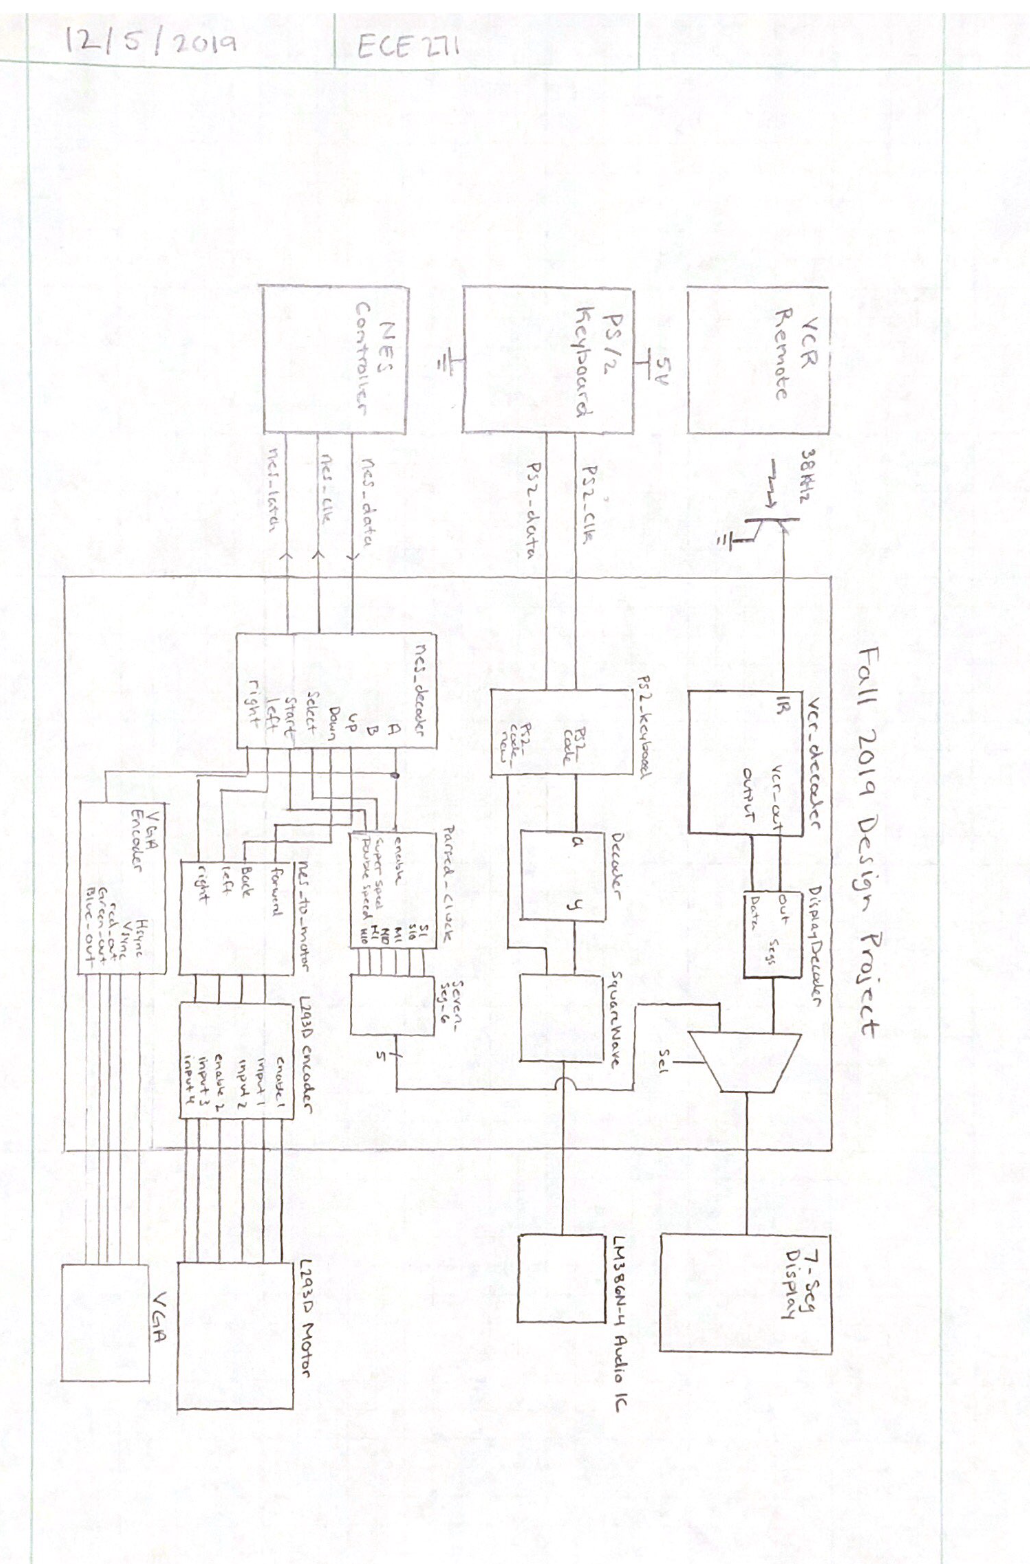
\includegraphics[width=.8\textwidth]{images/project_description.png}
	\caption{Top Level Diagram for the project. The Diagram shows all the Functional Units used in the project and how they are connected from input to output.}
  \label{fig:description}
\end{figure}

\begin{figure}[h]
  \centering
    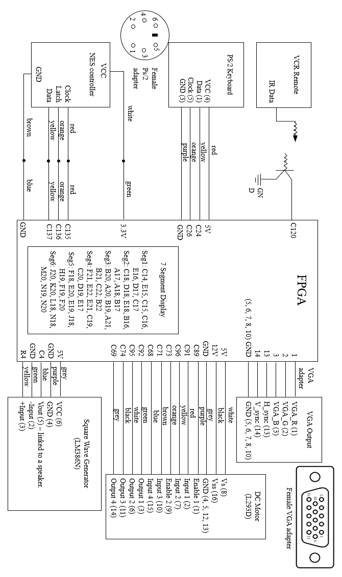
\includegraphics[width=.8\textwidth]{images/hardware_diagram.png}
	\caption{The hardware diagram shows which pins are used on the FPGA, module boards, and relevant supply voltages for the different pieces of hardware used in the system.}
    \label{fig:hardware}
\end{figure}



\clearpage



\section{High Level Description}
This section provides a Top level introduction to the project. The input and output specifications are provided below, as well as a toplevel diagram in \textbf{Figure 3}, and the simulation results in \textbf{Figure 4}.


\begin{itemize}
  \item \textbf{Inputs:  } The Top Level of the project has 7 inputs: switch1, switch2, system\_reset\_button, nes\_data, clock\_50MHz, ps2\_clk, and ps2\_data.
    \begin{itemize}
      \item \textbf{switch1: } switch1 is used to enable the square wave generator unit connected to the PS2 Keyboard.
      \item \textbf{switch2: }
      \item \textbf{system\_reset\_button: } system\_reset\_button is an active high signal used to reset the nes\_decoder, vga\_encoder, and parsed\_clock Functional Units.
      \item \textbf{nes\_data: } the input signal from the NES Controller into the nes\_decoder Functional Unit.
      \item \textbf{clock\_50MHz: } the internal clock on the FPGA that is used generate all the other clock signals used in the top level.
      \item \textbf{ps2\_clk: } the clock signal driving the ps\_2\_keyboard Functional Unit.
      \item \textbf{ps2\_data: } the input signal from the PS2 Keyboard into the ps2\_keyboard functional unit.
    \end{itemize}
  \item \textbf{Outputs: } The Top level has outputs going to the NES Controller, the seven segment pins in the FPGA, the L293D DC Controller, the square wave generator, and the VGA pins.
\end{itemize}

\begin{figure}[h]
  \centering
    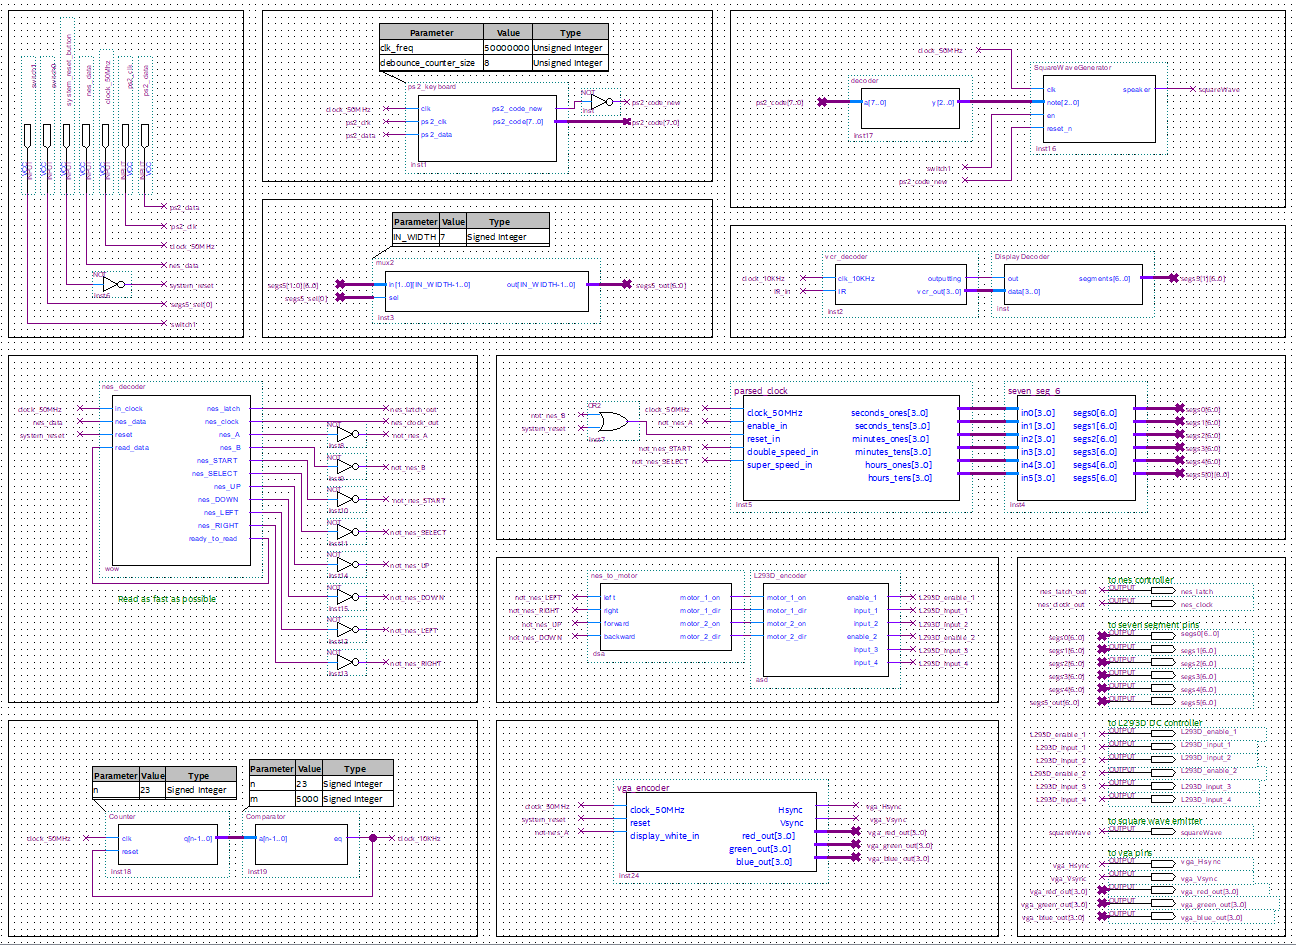
\includegraphics[width=.98\textwidth]{images/top_level.png}
	\caption{The top level design for the  project.}
    \label{fig:top-level}
\end{figure}

\clearpage


\begin{figure}[h]
  \centering
  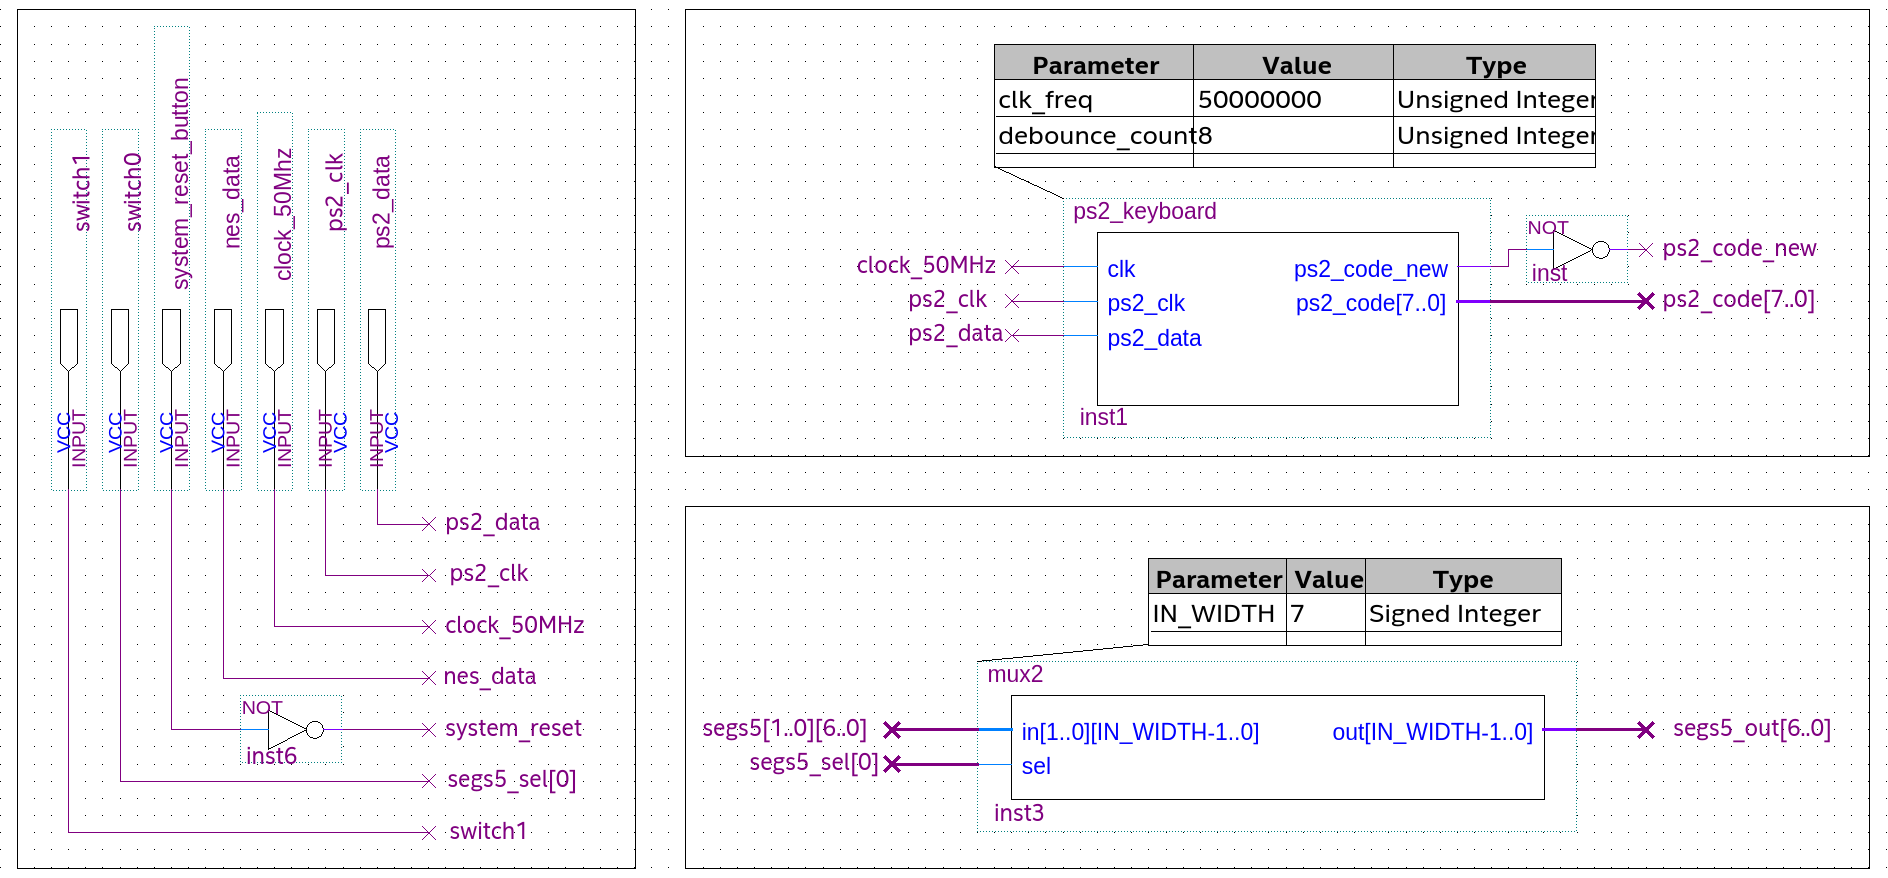
\includegraphics[width=.8\textwidth]{images/top_level_block_1.png}
  \subcaption{Block 1 of top level. Includes the inputs to the Top Level of the design, the ps2\_keyboard Functional unit, and the Multiplexer Functional Unit that controls input to the seven segment display.}
  \label{fig:top-level-block-1}
\end{figure}

\begin{figure}[h]
  \centering
  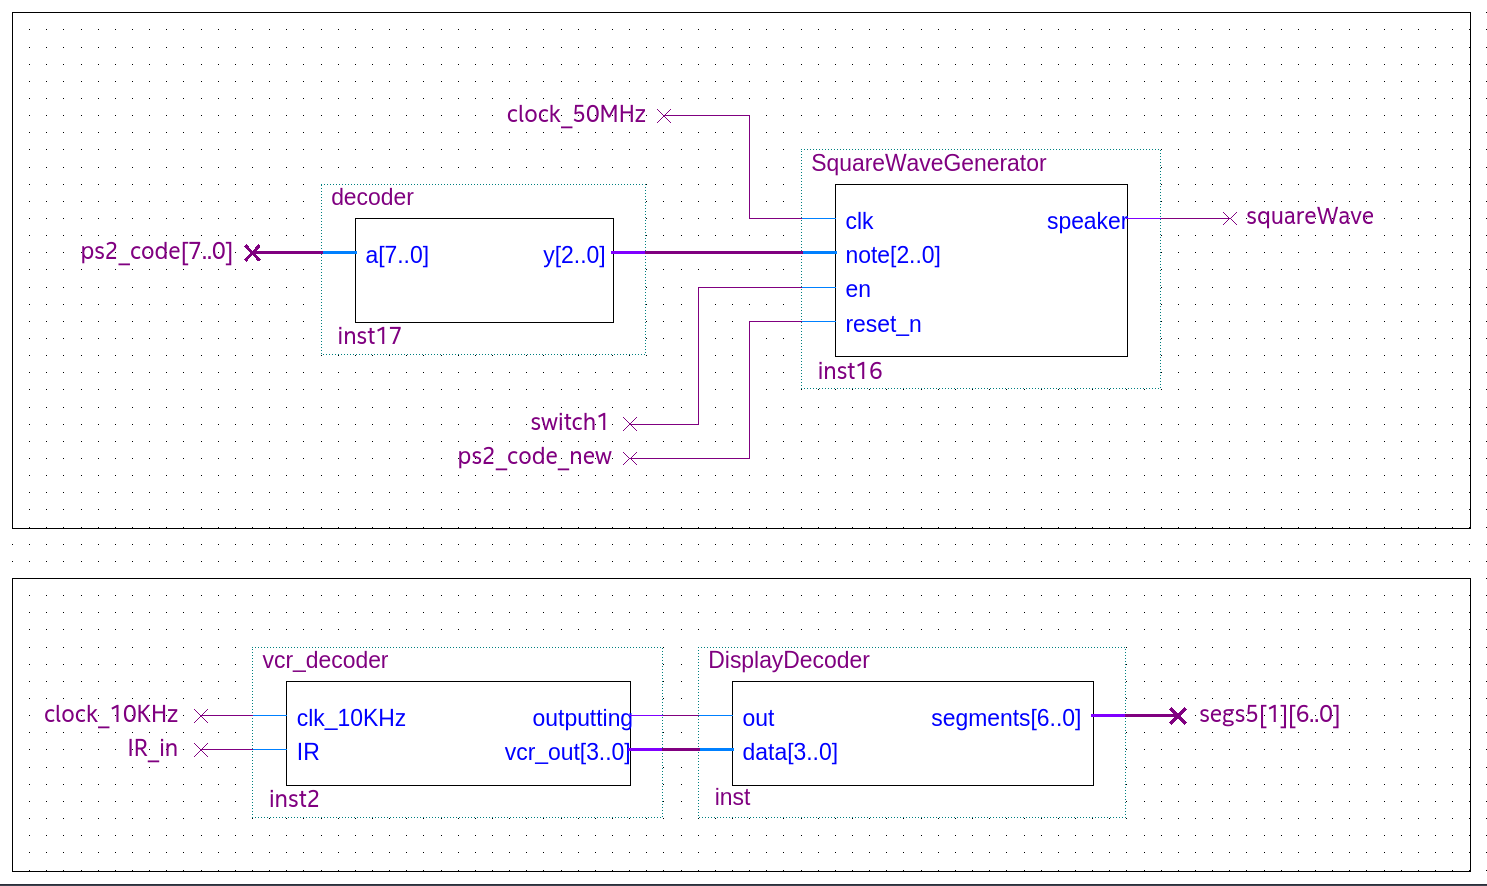
\includegraphics[width=.8\textwidth]{images/top_level_block_2.png}
  \subcaption{Block 2 of top level. Includes the decoder for the ps2\_keyboard functional unit, the square wave generator functional unit, the vcr\_decoder functional unit, and the DislayDecoder functional unit.}
  \label{fig:top-level-block-2}
\end{figure}

\begin{figure}[h]
  \centering
  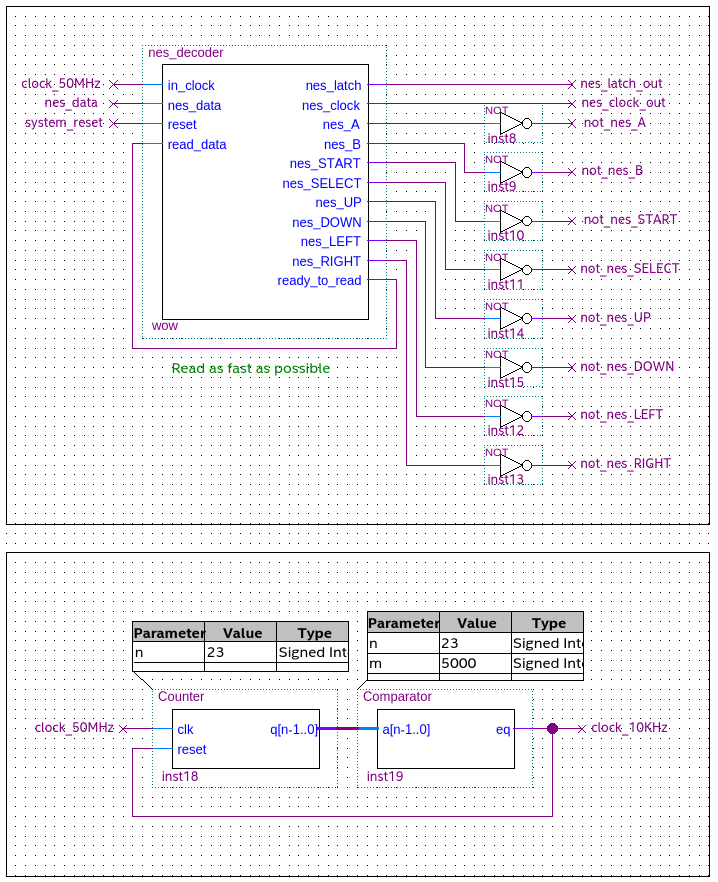
\includegraphics[width=.8\textwidth]{images/top_level_block_3.png}
  \subcaption{Block 3 of top level. Includes the nes\_decoder functional unit and the Counter and Comparator functional units used to generate the clock signal for the vcr\_decoder}
  \label{fig:top-level-block-3}
\end{figure}

\begin{figure}[h]
  \centering
  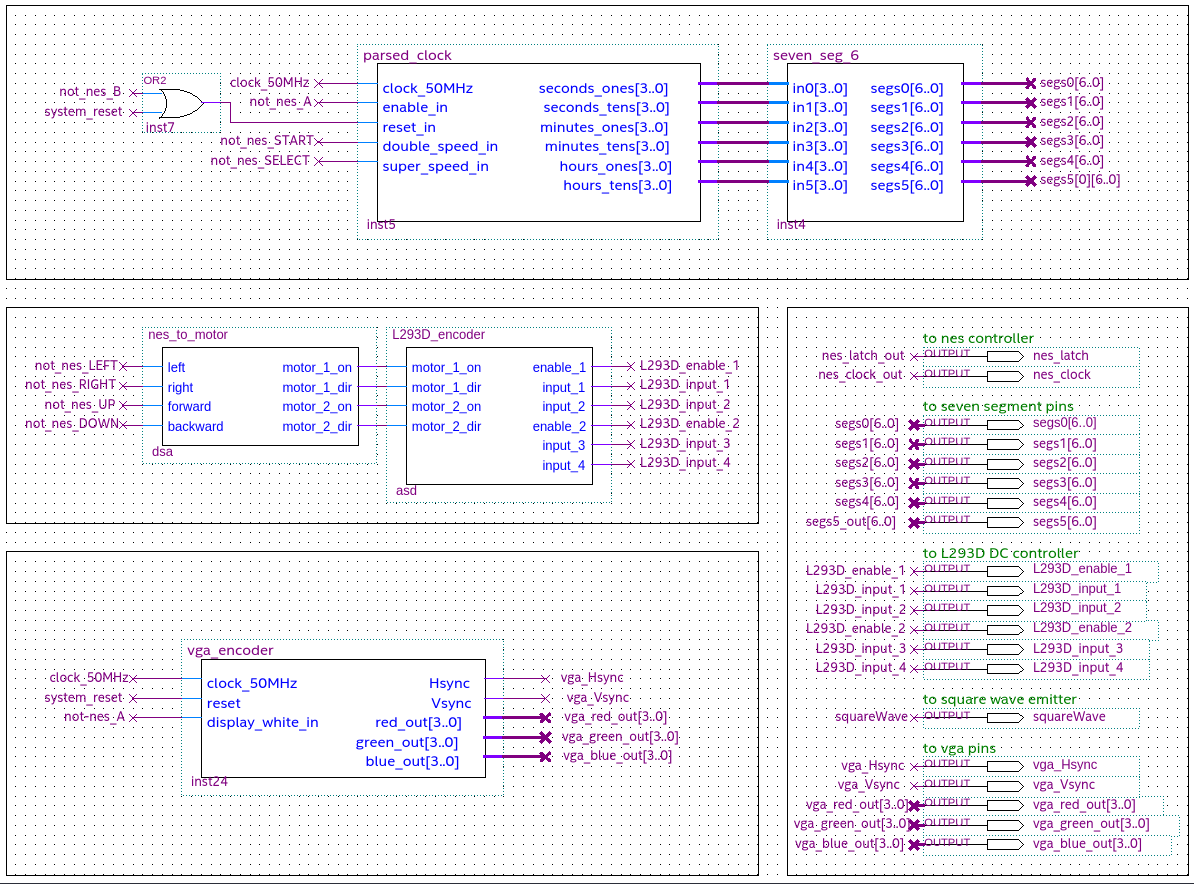
\includegraphics[width=.8\textwidth]{images/top_level_block_4.png}
  \subcaption{Block 4 of top level. Includes the parsed\_clock, seven\_seg\_6, nes\_to\_motor, L293D\_Encoder, and vga\_endocder functional units. In addition, it includes the outputs for the Top Level of the project.}
  \label{fig:top-level-block-4}
\end{figure}


\begin{figure}[h]
  \centering
    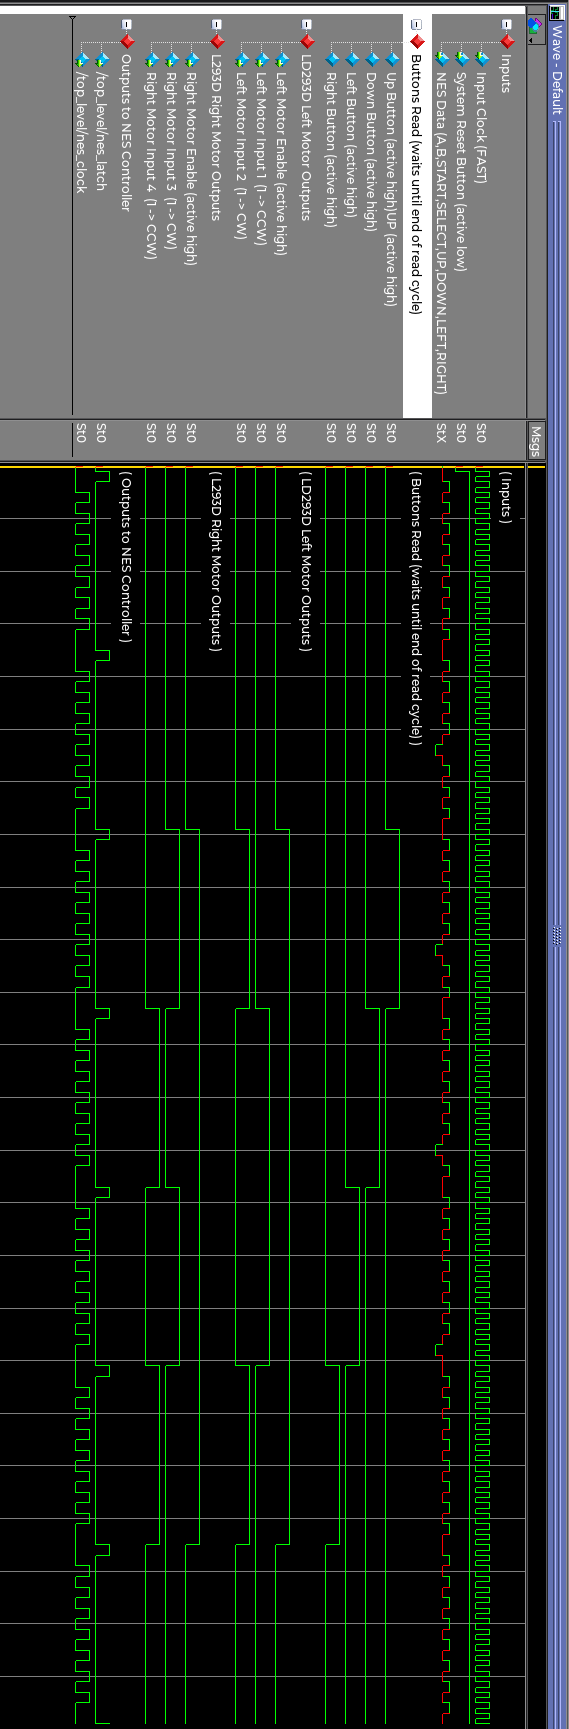
\includegraphics[height=0.98\textheight]{sims/top_level_motor_sim.png}
	\caption{The simulation results for the L293D DC Motor in the Top Level.}
    \label{fig:top-level-sim}
\end{figure}

\begin{figure}[h]
  \centering
    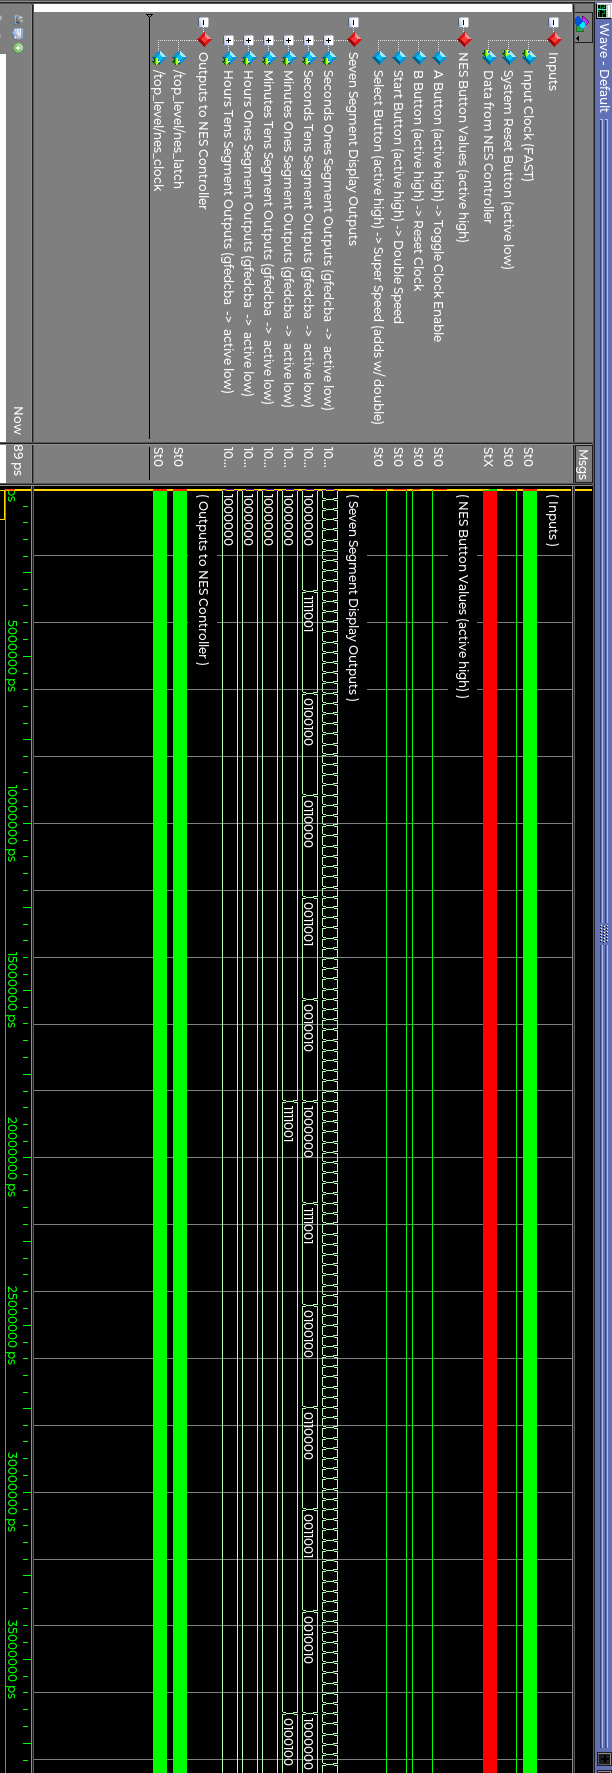
\includegraphics[height=0.98\textheight]{sims/top_level_clock_sim_1.png}
	\caption{The simulation results for the NES Controller to seven segment display in Top Level.}
    \label{fig:top-level-sim}
\end{figure}

\begin{figure}[h]
  \centering
    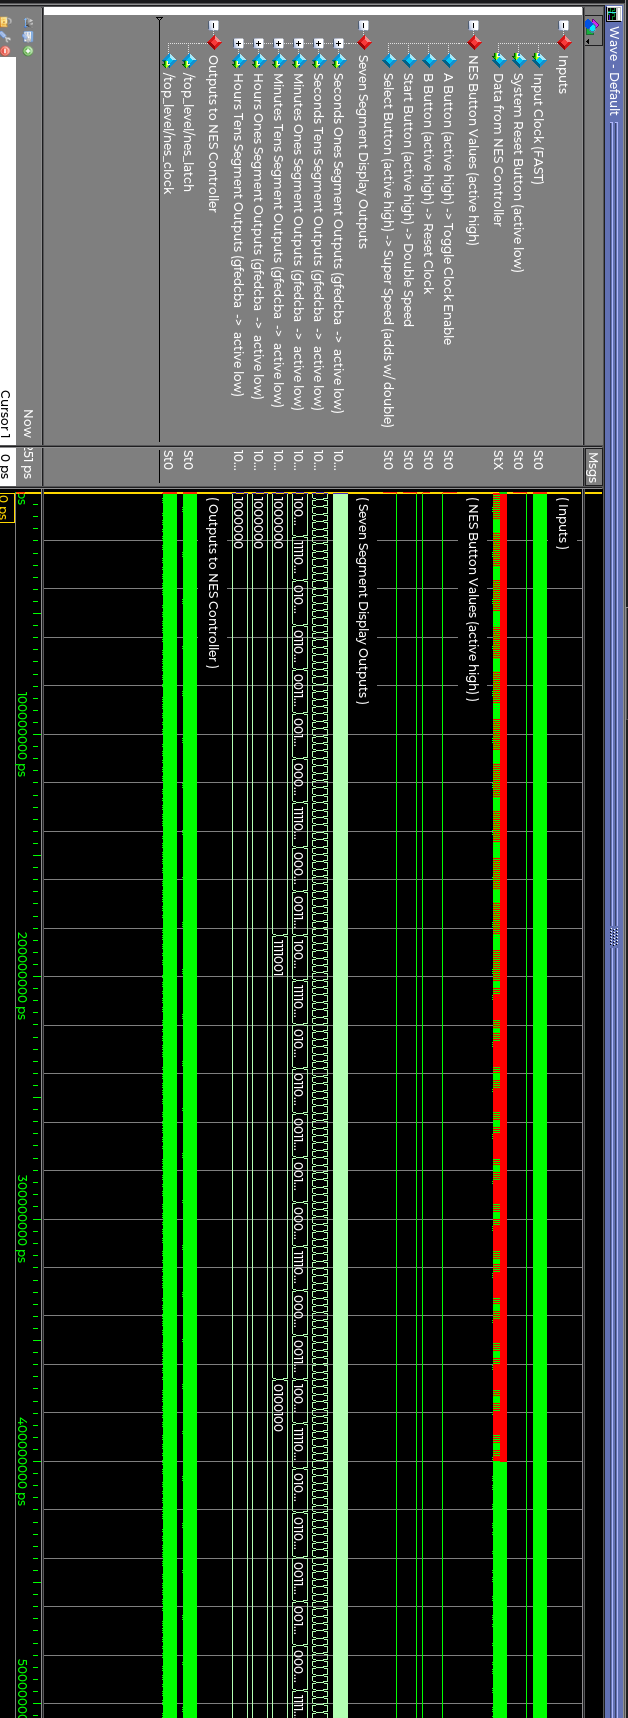
\includegraphics[height=0.98\textheight]{sims/top_level_clock_sim_2.png}
	\caption{The simulation results for the NES Controller to seven segment display in Top Level.}
    \label{fig:top-level-sim}
\end{figure}

\begin{figure}[h]
  \centering
    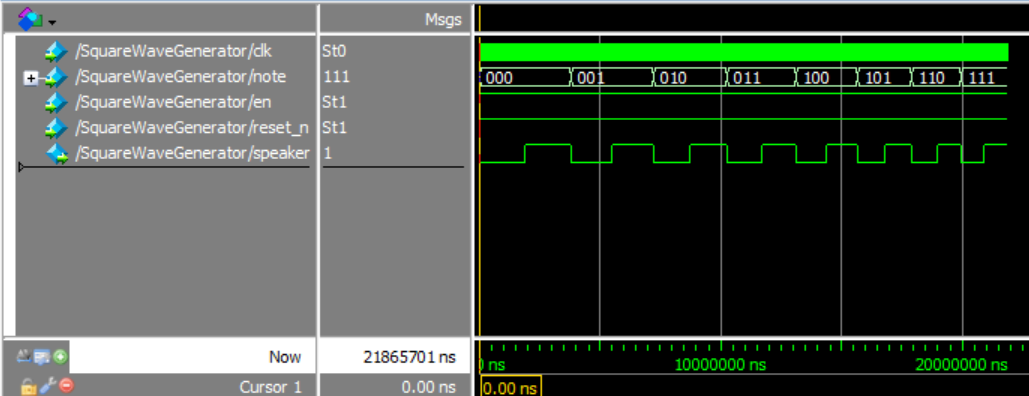
\includegraphics[width=0.98\textwidth]{sims/square_wave_generator/SquareWaveGenerator.png}
	\caption{The simulation results for the PS2 Keyboard to the LM386N-4 Audio IC in Top Level.}
    \label{fig:top-level-sim}
\end{figure}


\begin{figure}[t]
  \centering
  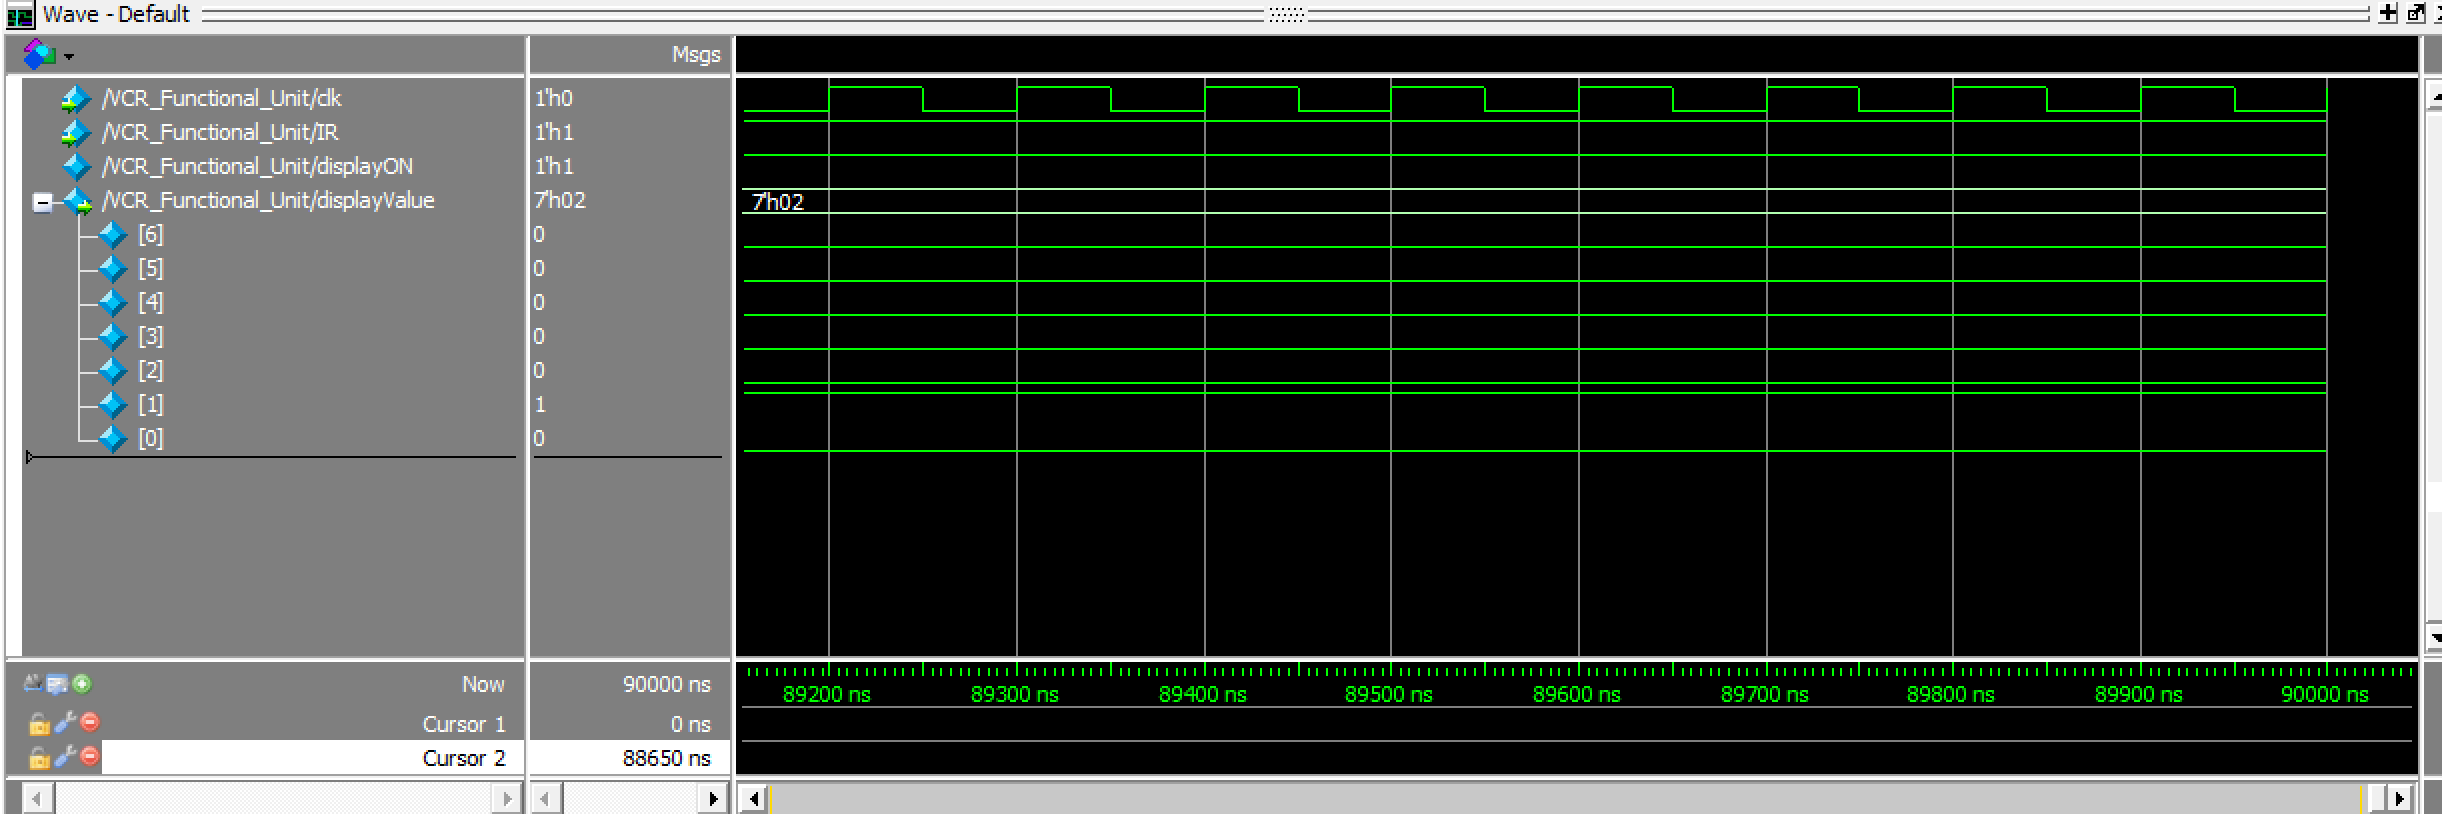
\includegraphics[width=.98\textwidth]{sims/vcr_testing/functionalUnitTest/FunctionalUnitTest_6.png}
  \caption{The Simulation results for Top Level VCR output with expected value of 6.}
  \label{fig:top-level-block-1}
\end{figure}

\begin{figure}[t]
  \centering
  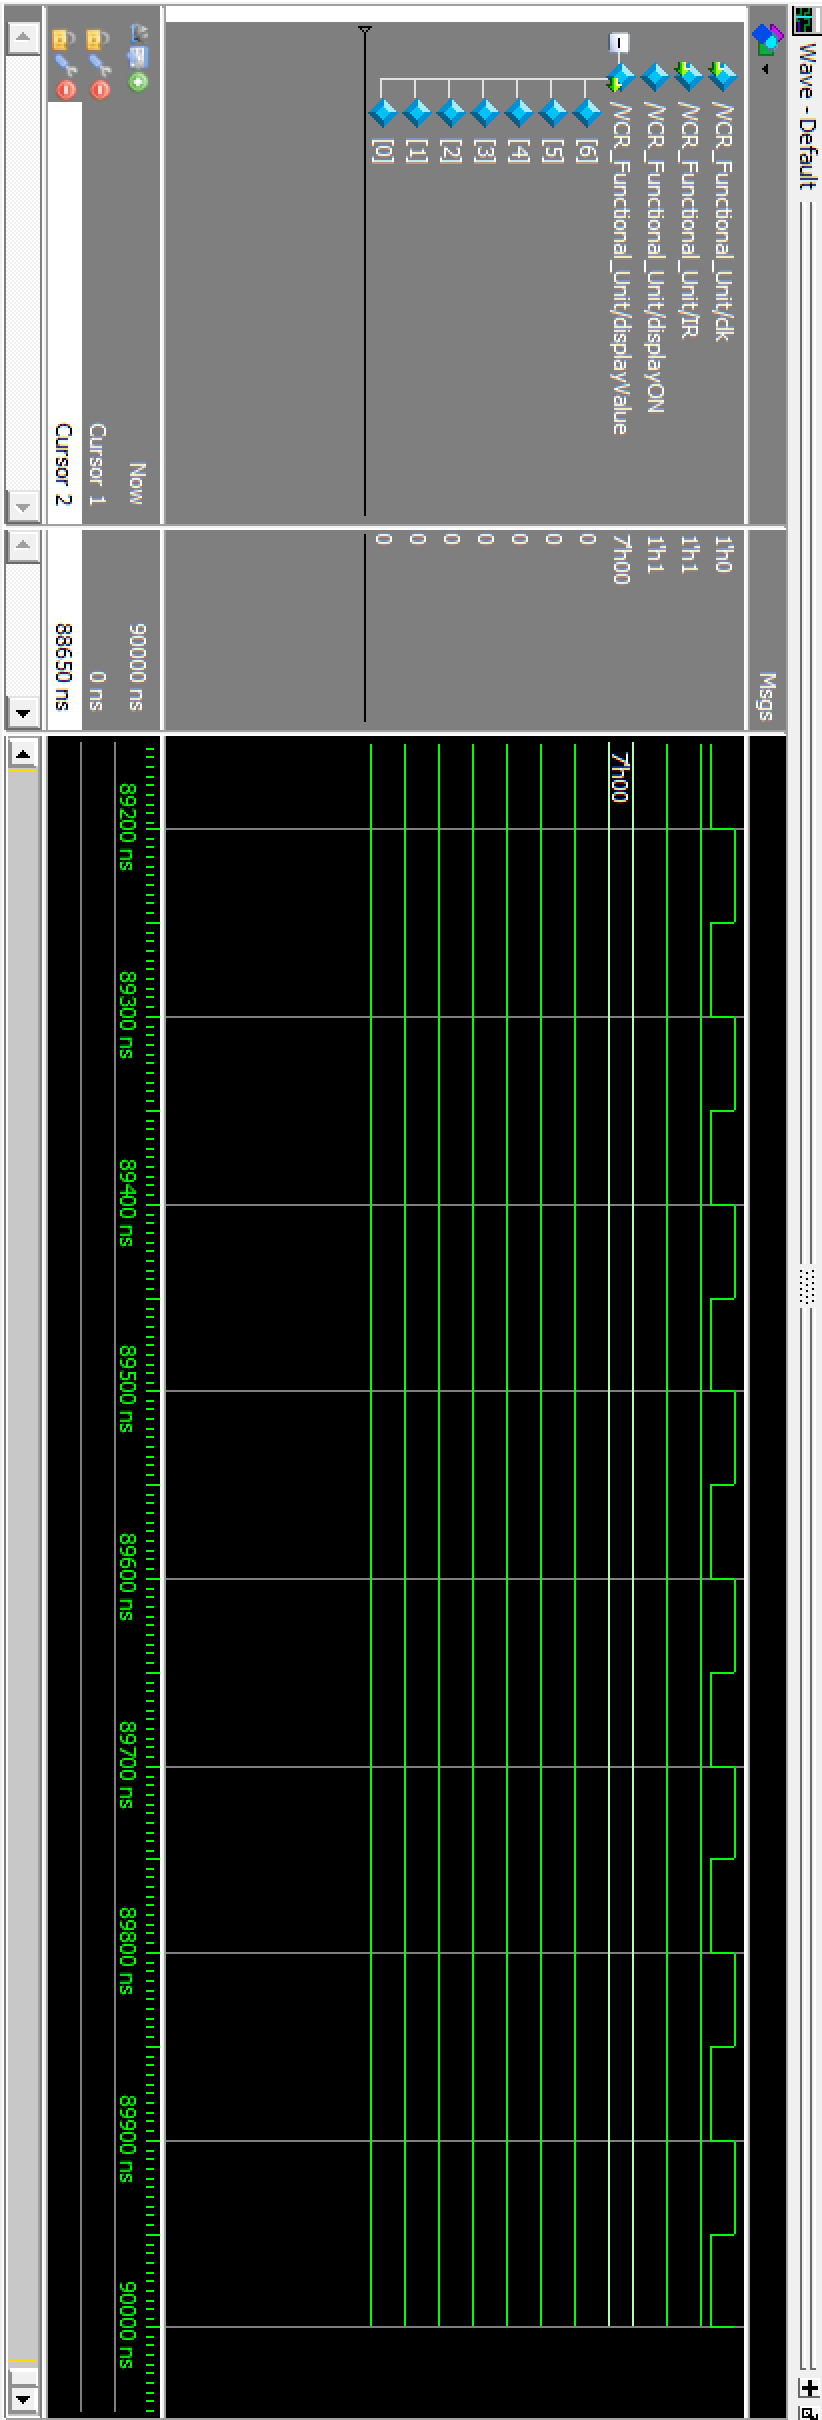
\includegraphics[width=.98\textwidth]{sims/vcr_testing/functionalUnitTest/FunctionalUnitTest_8.png}
  \caption{The Simulation results for Top Level VCR output with expected value of 8.}
  \label{fig:top-level-block-1}
\end{figure}


\FloatBarrier

The following subsections will discuss the inputs, outputs, designs, and simulation results of all elements of the design at two levels of scrutiny: functional units and individual blocks of digital logic.



\clearpage


%% Functional Subsections
\catcode`\_=13
\def_{\textunderscore}
\subsection{decoder Functional Unit}
\catcode`_=8
The decoder block decodes the data from the PS/2 keyboard to the three-bit data. To match the keys in keyboard from a to t with the piano notes from middle C to the upper octave C, the hexadecimal code of the keyboard is converted to 3-bit data as shown in the simulation.  The logic symbol follows in \textbf{Figure 15}.  The simulation results follow in \textbf{Figure 16}.
\begin{itemize}
\item \textbf{Inputs:  } The decoder block has one input, a[7..0]. It indicates the input 8-bit data, which is the make code for keys on the keyboard.
\item \textbf{Outputs: } The decoder block has one input, y[2..0]. It is converted from 8-bit to 3-bit data and is used to determine the note to generate.
\end{itemize}
\begin{figure}[h]
\centering
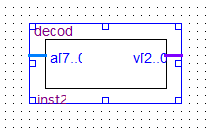
\includegraphics[width=.48\textwidth]{functional_units/decoder/decoder_symbol.png}
\caption{The block symbol of the decoder functional unit used in the final design.}
\end{figure}
\begin{figure}[h]
\centering
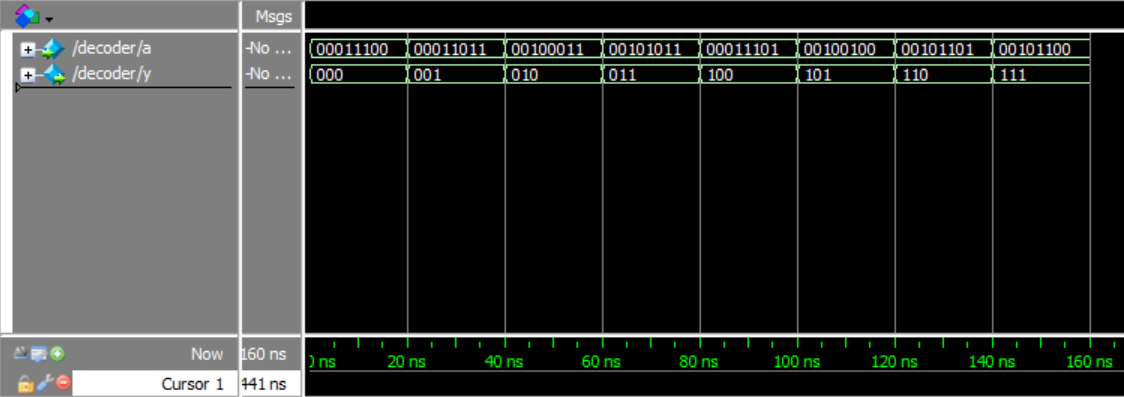
\includegraphics[width=.98\textwidth]{functional_units/decoder/decoder_sim.png}
\caption{The simulation results for the decoder module.}
\end{figure}
\clearpage

\catcode`\_=13
\def_{\textunderscore}
\subsection{seven\_seg\_6 Functional Unit}
\catcode`_=8
The seven\_seg\_6 module takes in six 4-bit binary values and converts them into the signals required to display each number (which will never exceed 9 in this design) on the FPGA's seven segment display. In this design, these inputs come directly from the parsed\_clock module that is controlled by the nes controller, and all but the most significant bit of these seven segment data lines go directly to the FPGA's seven segment display. In this design, either the most significant bit of the parsed\_clock OR the output of the vcr\_decoder are displayed on the seven segment display's most leftmost digit, depending on the state of the switch0 design input (determined by the mux2 submoduele of the vcr\_decoder module). A block diagram follows in \textbf{Figure 17}.  The logic symbol follows in \textbf{Figure 18}.  The simulation results follow in \textbf{Figure 19}.
\begin{itemize}
\item \textbf{Inputs:  } Six 4-bit binary value inputs from the parsed\_clock module that describe the one's and ten's places of the seconds, minutes, and hours of the clock. These values never exceed 59 seconds, 59 minutes, and 23 hours, so each place can only be 0-9 and failure of the sevenseg submodules due to overflow is impossible.
\item \textbf{Outputs: } Six 7-bit outputs describing how to display each input on a seven segment display. All but the most significant bit of these seven segment data lines go directly to the FPGA's seven segment display. In this design, either the most significant bit of the parsed\_clock OR the output of the vcr\_decoder are displayed on the seven segment display's most leftmost digit, depending on the state of the switch0 design input (based by the mux2 submoduele of the vcr\_decoder module).
\end{itemize}
\begin{figure}[h]
\centering
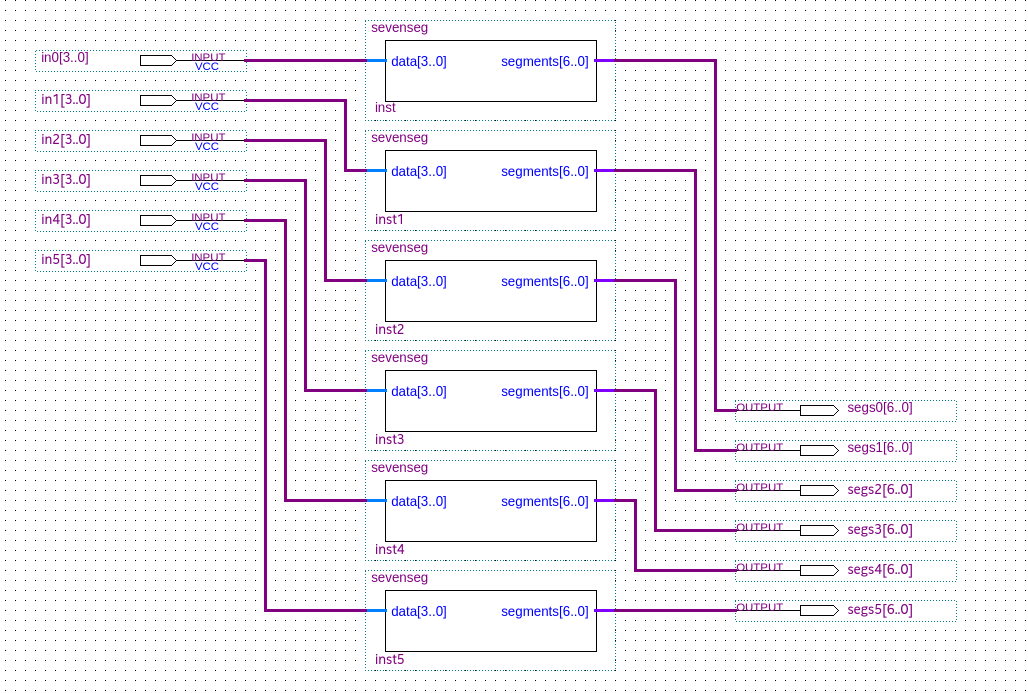
\includegraphics[width=.8\textwidth]{functional_units/seven_seg_6/seven_seg_6_block.png}
\caption{The logic design of the seven\_seg\_6 functional unit used in the final design.}
\end{figure}
\begin{figure}[h]
\centering
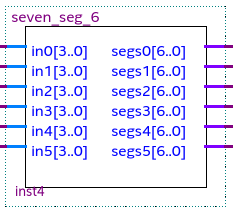
\includegraphics[width=.48\textwidth]{functional_units/seven_seg_6/seven_seg_6_symbol.png}
\caption{The block symbol of the seven\_seg\_6 functional unit used in the final design.}
\end{figure}
\begin{figure}[h]
\centering
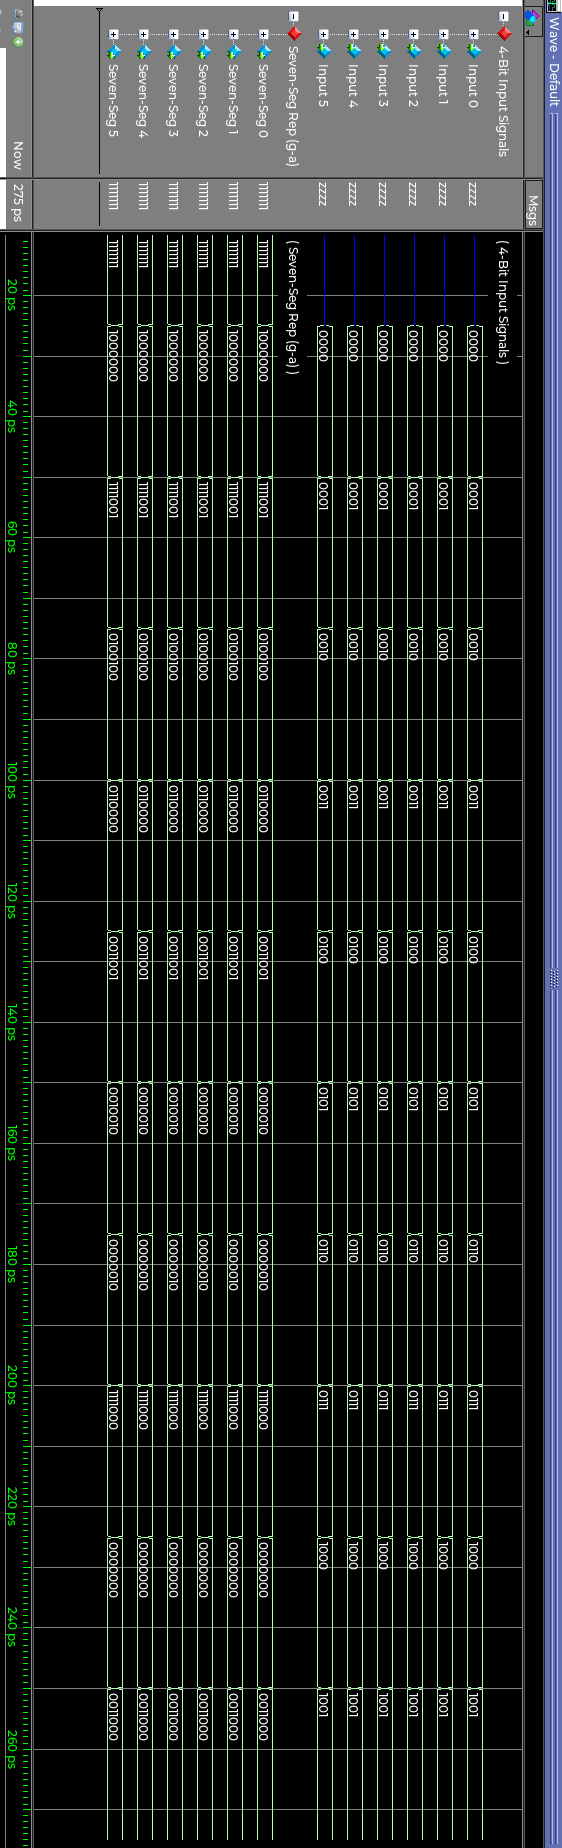
\includegraphics[width=.98\textwidth]{functional_units/seven_seg_6/seven_seg_6_sim.png}
\caption{The simulation results for the seven\_seg\_6 module.}
\end{figure}
\clearpage

\catcode`\_=13
\def_{\textunderscore}
\subsubsection{sevenseg Component Block}
\catcode`_=8
The sevenseg submodule converts a single 4-bit value between 0 and 9 into a 7-bit output describing how to display the input on a seven segment display. In this design, six of these sevenseg blocks are used in the seven\_seg\_6 module. The logic symbol follows in \textbf{Figure 20}.  The simulation results follow in \textbf{Figure 21}.
\begin{itemize}
\item \textbf{Inputs:  } A single 4-bit value between 0 and 9 to be converted in to a seven segment representation (data[3:0]).
\item \textbf{Outputs: } A 7-bit output describing how to display the input value on a seven segment display (segments[6:0]).
\end{itemize}
\begin{figure}[h]
\centering
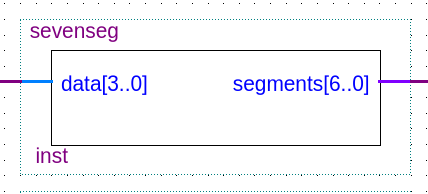
\includegraphics[width=.48\textwidth]{functional_units/seven_seg_6/individual_blocks/sevenseg_symbol.png}
\caption{The block symbol of the sevenseg module used in the seven\_seg\_6 functional unit.}
\end{figure}
\begin{figure}[h]
\centering
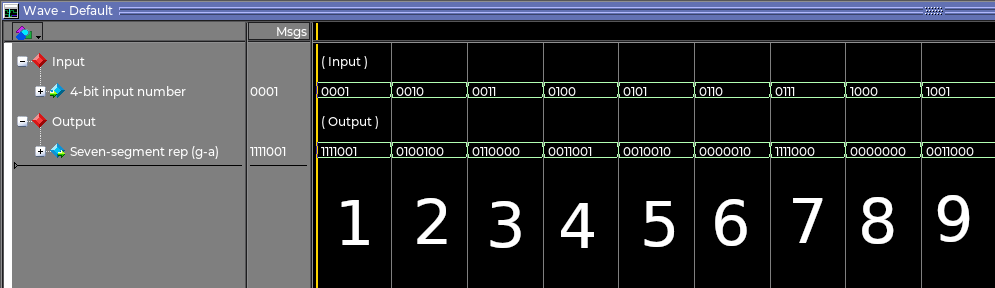
\includegraphics[width=.98\textwidth]{functional_units/seven_seg_6/individual_blocks/sevenseg_sim.png}
\caption{The simulation results for the sevenseg module used in the seven\_seg\_6 functional unit.}
\end{figure}
\clearpage

\catcode`\_=13
\def_{\textunderscore}
\subsection{L293D\_encoder Functional Unit}
\catcode`_=8
The L293D\_encoder functional unit converts internal system values describing how two motors should be driven to data in the format of the L293D DC motor controller. It is connected to these outputs, and takes its inputs from the nes\_to\_motor module. The logic symbol follows in \textbf{Figure 22}.  The simulation results follow in \textbf{Figure 23}.
\begin{itemize}
\item \textbf{Inputs:  } Whether motors 1 (left) and 2 (right) should be spinning (motor\_1\_on and motor\_2\_on); and which direction each motor should spin if also enabled, where logic high correlates to clockwise motion (motor\_1\_dir and motor\_2\_dir for each motor, respectively).
\item \textbf{Outputs: } The signals that the L293D DC motor controller takes in as inputs: enable\_1 and enable\_2 that describe whether motor 1 (left) and motor 2 (right) should be run; input\_1 and input\_2 which are always opposite signals describing the direction of rotation of the first (left) motor (where input\_1 high and input\_2 low correlates with clockwise rotation, for example); and input\_3 and input\_4 which are always opposite signals describing the direction of rotation of the second (right) motor (where input\_1 high and input\_2 low correlates with clockwise rotation, for example).
\end{itemize}
\begin{figure}[h]
\centering
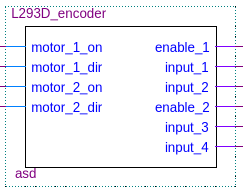
\includegraphics[width=.48\textwidth]{functional_units/L293D_encoder/L293D_encoder_symbol.png}
\caption{The block symbol of the L293D\_encoder functional unit used in the final design.}
\end{figure}
\begin{figure}[h]
\centering
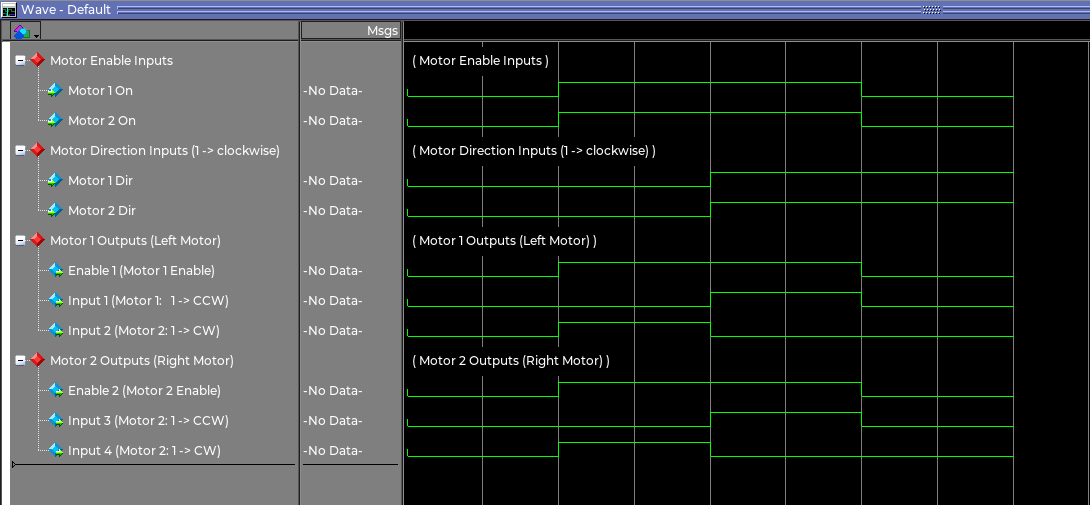
\includegraphics[width=.98\textwidth]{functional_units/L293D_encoder/L293D_encoder_sim.png}
\caption{The simulation results for the L293D\_encoder module.}
\end{figure}
\clearpage

\catcode`\_=13
\def_{\textunderscore}
\subsection{Counter Functional Unit}
\catcode`_=8
The Counter Functional Unit increments a counter on every rising edge of the input clock signal. This is used to generate a 10 KHz clock signal to drive the vcr\_decoder Functional Unit. The logic symbol follows in \textbf{Figure 24}.  The simulation results follow in \textbf{Figure 25}.
\begin{itemize}
\item \textbf{Inputs:  } The Counter Functional Unit has 2 inputs: clk and reset. clk is the 50 MHz FPGA clock that is used to drive the counter. reset is an input signal that resets the counter to 0.
\item \textbf{Outputs: } The Counter Functional Unit has 1 output: q. q is a 23-bit value with the current value of the counter.
\end{itemize}
\begin{figure}[h]
\centering
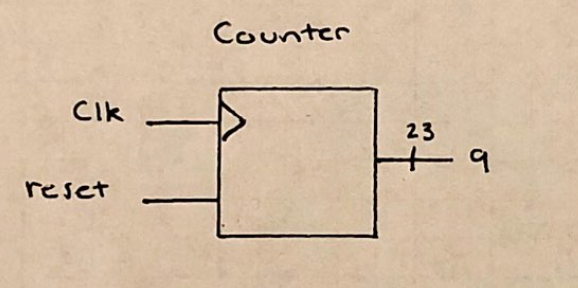
\includegraphics[width=.48\textwidth]{functional_units/Counter/Counter_symbol.png}
\caption{The block symbol of the Counter functional unit used in the final design.}
\end{figure}
\begin{figure}[h]
\centering
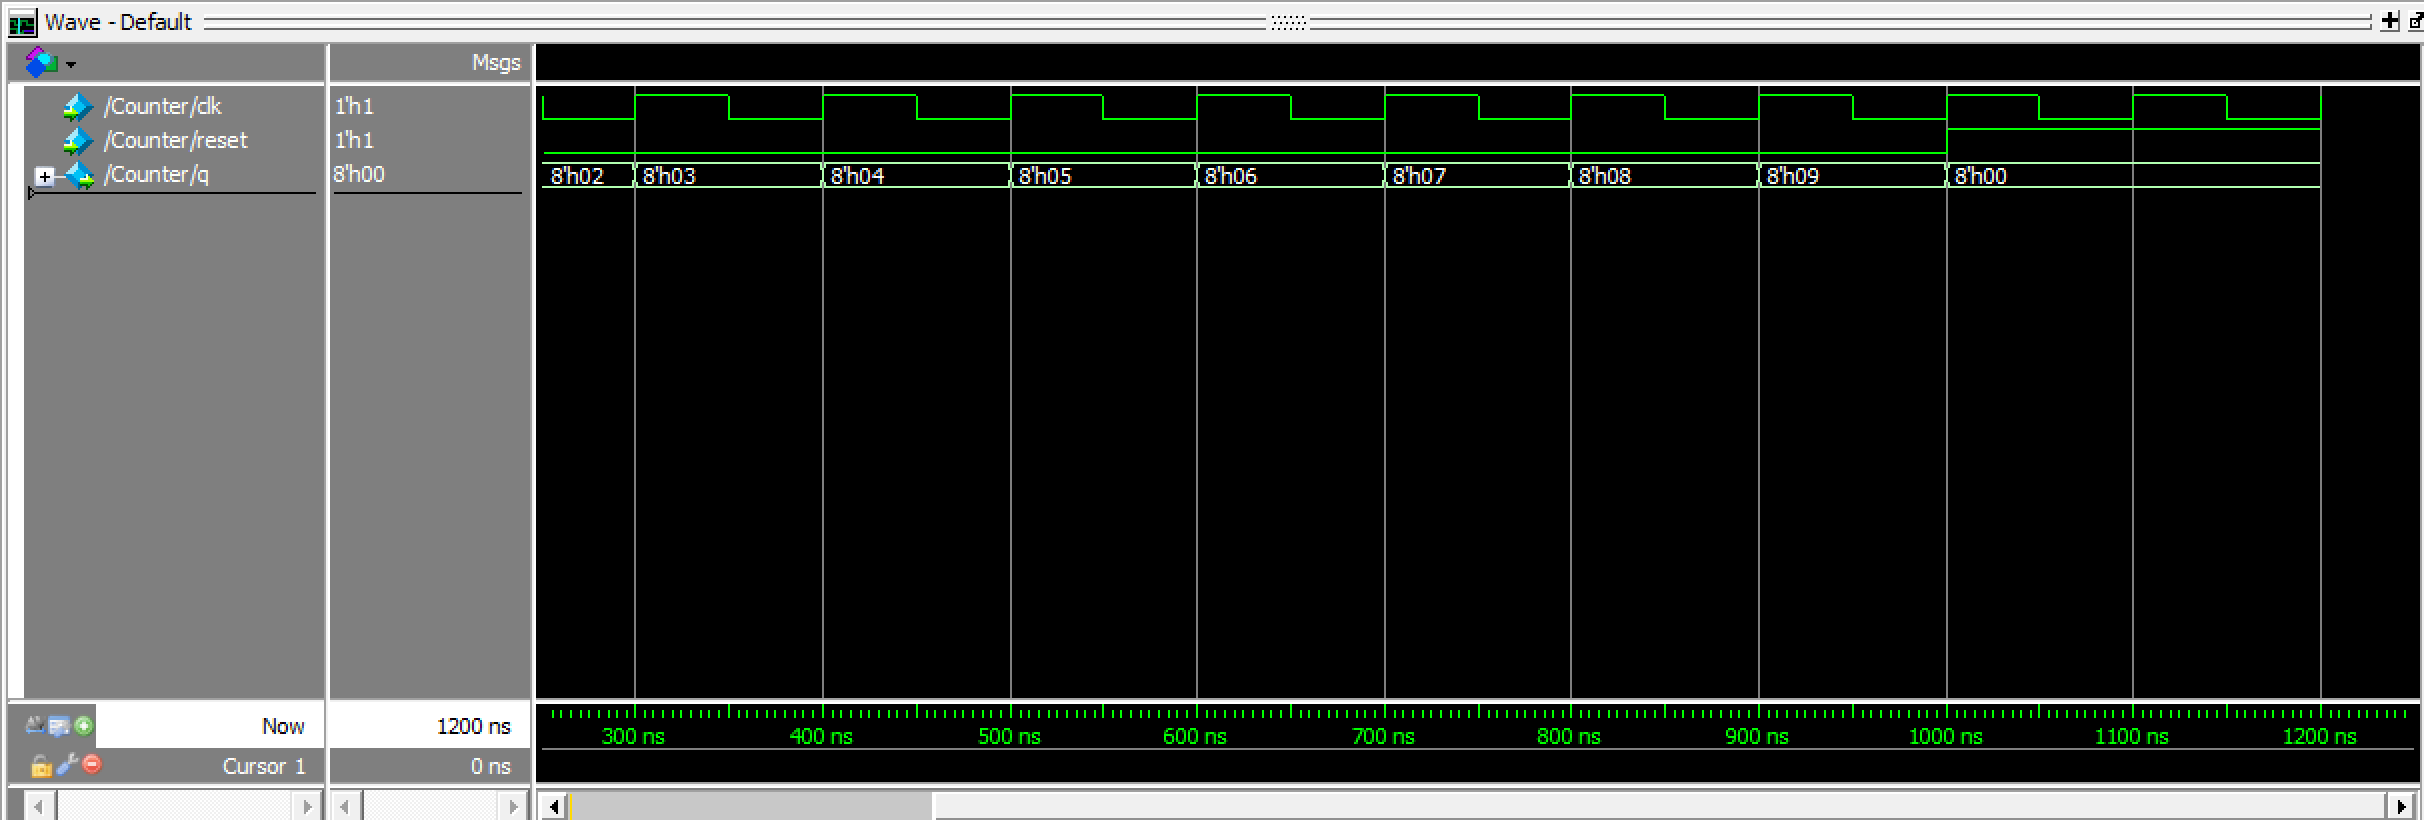
\includegraphics[width=.98\textwidth]{functional_units/Counter/Counter_sim.png}
\caption{The simulation results for the Counter module.}
\end{figure}
\clearpage

\catcode`\_=13
\def_{\textunderscore}
\subsection{vga\_encoder Functional Unit}
\catcode`_=8
Intro text. A block diagram follows in \textbf{Figure 26}.  The logic symbol follows in \textbf{Figure 27}.
\begin{itemize}
\item \textbf{Inputs:  } Input text.
\item \textbf{Outputs: } Output text.
\end{itemize}
\begin{figure}[h]
\centering
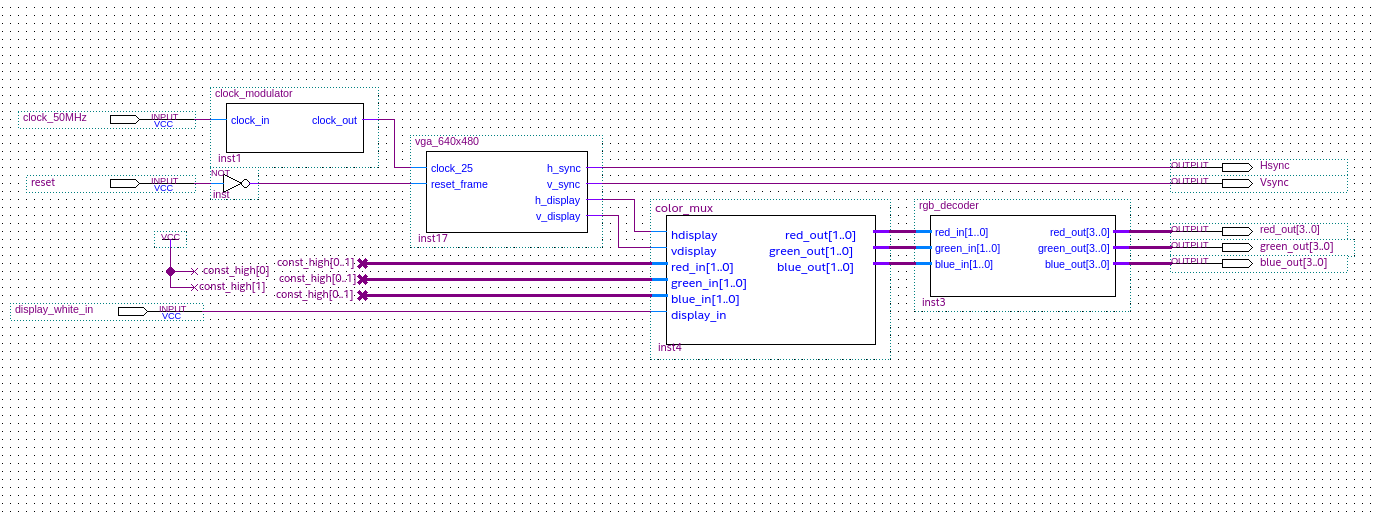
\includegraphics[width=.8\textwidth]{functional_units/vga_encoder/vga_encoder_block.png}
\caption{The logic design of the vga\_encoder functional unit used in the final design.}
\end{figure}
\begin{figure}[h]
\centering
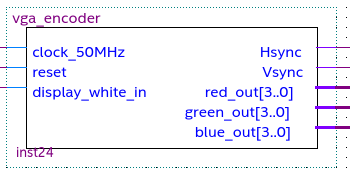
\includegraphics[width=.48\textwidth]{functional_units/vga_encoder/vga_encoder_symbol.png}
\caption{The block symbol of the vga\_encoder functional unit used in the final design.}
\end{figure}
\clearpage

\catcode`\_=13
\def_{\textunderscore}
\subsection{vcr\_decoder Functional Unit}
\catcode`_=8
The vcr\_decoder module converts an IR signal sent from a VCR remote into a decimal value between 0 and 9. The logic symbol follows in \textbf{Figure 28}.
\begin{itemize}
\item \textbf{Inputs:  } The vcr\_decoder module has two inputs, clk and IR. clk is a 10 KHz clock signal that is used to drive the module. IR is the Infrared signal coming from the VCR remote that will be translated by the module.
\item \textbf{Outputs: } The vcr\_decoder module has a single output, displayValue, which is the 0-9 representing the IR signal that was received by the module as input.
\end{itemize}
\begin{figure}[h]
\centering
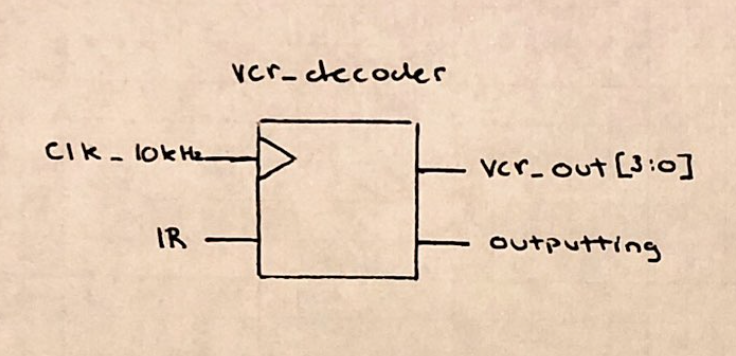
\includegraphics[width=.48\textwidth]{functional_units/vcr_decoder/vcr_decoder_symbol.png}
\caption{The block symbol of the vcr\_decoder functional unit used in the final design.}
\end{figure}
\clearpage

\catcode`\_=13
\def_{\textunderscore}
\subsubsection{mux2 Component Block}
\catcode`_=8
The mux2 individual block is used to choose whether the seven segment display shows the output of the nes decoder functional unit or the vcr\_decoder functional unit.
\begin{itemize}
\item \textbf{Inputs:  } The mux2 individual block has 2 inputs: sel and in. in is the input signal which is 2 bits wide. sel is used to select which of the values goes to the output.
\item \textbf{Outputs: } The mux2 individual block has 1 output: out. This is the value that is selected by the sel input signal.
\end{itemize}
\clearpage

\catcode`\_=13
\def_{\textunderscore}
\subsubsection{ReadState Component Block}
\catcode`_=8
The ReadState Individual Block is used to implement the READ state within the vcr\_decoder Module. The logic symbol follows in \textbf{Figure 29}.
\begin{itemize}
\item \textbf{Inputs:  } The ReadState Individual Block has 3 inputs: clk, IR, and start. clk is a 10 KHz clock that drives the ReadState block. IR is the infrared signal generated by the VCR remote on a given button push. Start is a control signal for the ReadState Individual Block. When start is 1, the block will operate.
\item \textbf{Outputs: } The ReadState Individual Block has 2 outputs: pushOutput and outputValue. pushOutput is a control signal that is used to communicate that the ReadState block is ready to output the value of outputValue. outputValue is the 32-bit value that identifies the IR signal that reciieved by the block.
\end{itemize}
\begin{figure}[h]
\centering
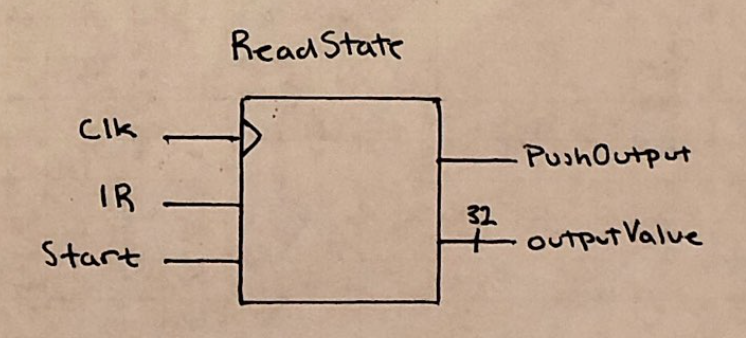
\includegraphics[width=.48\textwidth]{functional_units/vcr_decoder/individual_blocks/ReadState_symbol.png}
\caption{The block symbol of the ReadState module used in the vcr\_decoder functional unit.}
\end{figure}
\clearpage

\catcode`\_=13
\def_{\textunderscore}
\subsubsection{ShiftRegister Component Block}
\catcode`_=8
The ShiftRegister Individual Block is used to store the 32-bit IR signal value bit by bit as as it is read in by the ReadState Module. The logic symbol follows in \textbf{Figure 30}.  The simulation results follow in \textbf{Figure 31}.
\begin{itemize}
\item \textbf{Inputs:  } The ShiftRegister Individual Block has five inputs. The first input is a clock signal, clk. On every rising edge of this clock signal, a new bit is shifted into the register. The second input is sin. This is the bit that is being shifted into the register. the third input is d. d is a 32-bit value which can be used to fully load the the shift register. The fourth input is load. When load is 1, the value stored at d is shifted into the register. The final input is reset, which clears the shift register's contents
\item \textbf{Outputs: } The ShiftRegister Individual Block has 2 outputs, q and sout. q is a 32-bit value that represents all the bits that have been shifted into the register. sout is the most significant bit in q.
\end{itemize}
\begin{figure}[h]
\centering
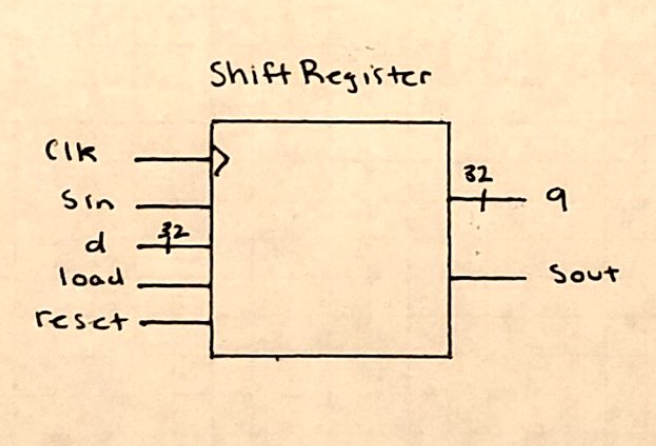
\includegraphics[width=.48\textwidth]{functional_units/vcr_decoder/individual_blocks/ShiftRegister_symbol.png}
\caption{The block symbol of the ShiftRegister module used in the vcr\_decoder functional unit.}
\end{figure}
\begin{figure}[h]
\centering
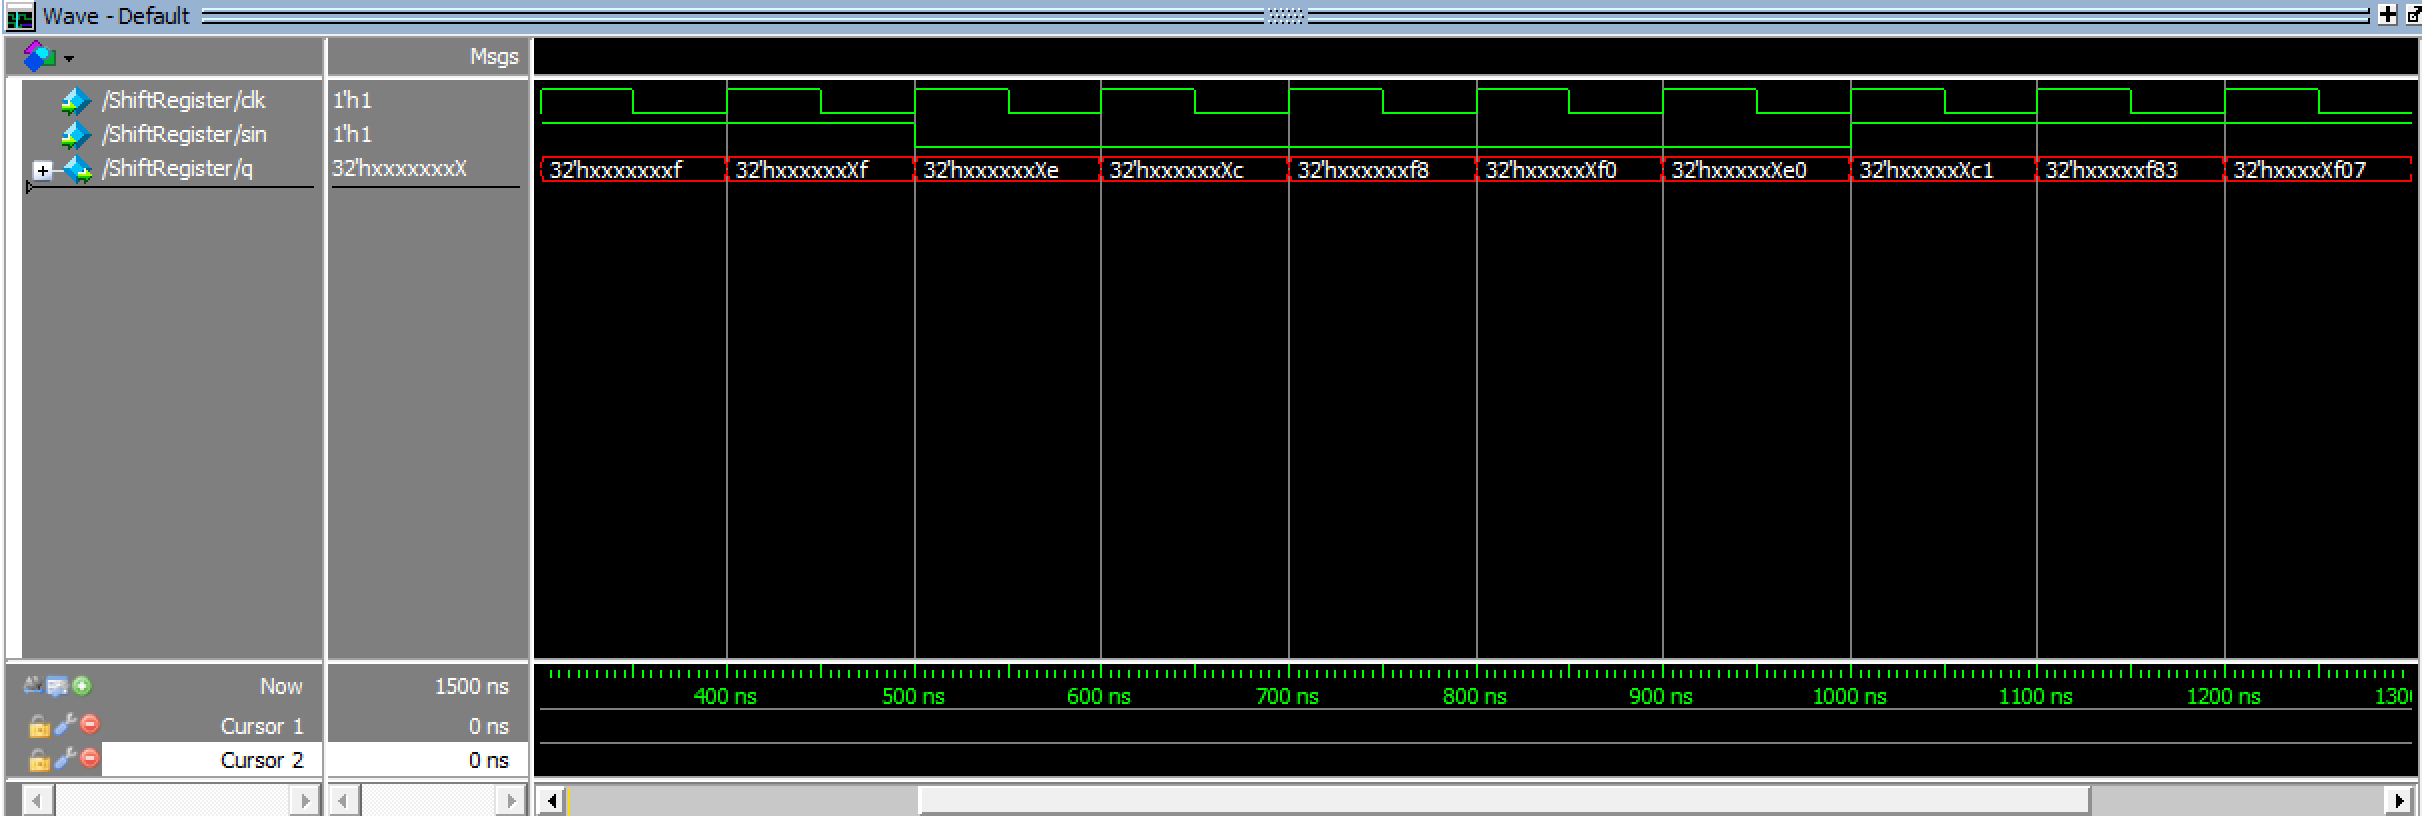
\includegraphics[width=.98\textwidth]{functional_units/vcr_decoder/individual_blocks/ShiftRegister_sim.png}
\caption{The simulation results for the ShiftRegister module used in the vcr\_decoder functional unit.}
\end{figure}
\clearpage

\catcode`\_=13
\def_{\textunderscore}
\subsubsection{signalDecoder Component Block}
\catcode`_=8
The SignalDecoder Individual Block is used to convert the 32-bit value generated by the ReadState Individual Block into a 4-bit value by 0 and 15 that indicated which button on the VCR remote was pressed.
\begin{itemize}
\item \textbf{Inputs:  } The SignalDecoder Individual Block takes a single 32-bit input that corresponds to the complete IR signal that was read in by the ReadState Individual Block.
\item \textbf{Outputs: } The SignalDecoder Individual Block outputs a 4-bit value betwee 0 and 15.
\end{itemize}
\clearpage

\catcode`\_=13
\def_{\textunderscore}
\subsection{ps2\_keyboard Functional Unit}
\catcode`_=8
PS/2 is an interface for keyboards and mice to PC via a 6-pin Mini-DIN connector. The system must provide the keyboard or mouse with 5V source and ground connections. Communication occurs over two wires, a clock line and a data line. The clock has a frequency between 10 kHz and 16.7 kHz. The data has a start bit, which is set as logic low, one byte of data, a parity bit, and a stop bit, which is set as logic high. Each bit is read on the falling edge of the clock signal. In the schematics, ps2\_data and ps2\_clk first synchronized and debounced. The data signal is then loaded to a shift register on falling edges of the PS/2 clock so that the flip flops can store the data. When the data transmission is finished and the clock remains high for more than 55us, the time longer than half of the worst-case PS/2 clock period, idle counter sends logic high to the AND gate. If there is no error and the signal from the idle counter is high, ps2\_code\_new becomes logic high indicating that the block is ready for the next signal. The ps2\_code[7..0] gets ps2\_word[8..1] because flip flops in that position contain the data. In the simulation, the waves indicate clock with 50MHz, ps2\_clk, ps2\_data, ps2\_code\_new, and ps2\_code[7..0] in sequence. The signals for ps2\_clk and ps2\_data are gotten from the csv file provided. After ps2\_word[10..0] stores the signal of ps2\_data at the falling edge of the ps2\_clk, ps2\_code\_new becomes 1 and ps2\_word[8..1] is sent to ps2\_code[7..0] if there is no error. The simulation figures below shows the simulation of pushing the keys of a, s, d, f, w, e, r, and t. The keys in PS/2 Keyboard have make code in hexadecimal. The code for the keys used in this project is 0x1C, 0x1B, 0x23, 0x2B, 0x1D, 0x24, 0x2D, and 0x2C respectively. The codes are shown in the simulation in the binary format.  A block diagram follows in \textbf{Figure 32}.  The logic symbol follows in \textbf{Figure 33}.  The simulation results follow in \textbf{Figure 34}.
\begin{itemize}
\item \textbf{Inputs:  } The PS/2 keyboard module has three inputs, clk, ps2\_data, ps2\_clk. The clk is the clock signal of 50MHz, ps2\_clk is the clock signal sent from the PS/2 keyboard to read the data, and the ps2\_data is the data sent from PS/2 keyboard.
\item \textbf{Outputs: } The PS/2 keyboard module has two outputs, ps2\_code[7..0], ps2\_code\_new. The ps2\_code[7..0] is the make code data for keys on the keyboard, and ps2\_code\_new indicates whether the module is ready for the next data or not.
\end{itemize}
\begin{figure}[h]
\centering
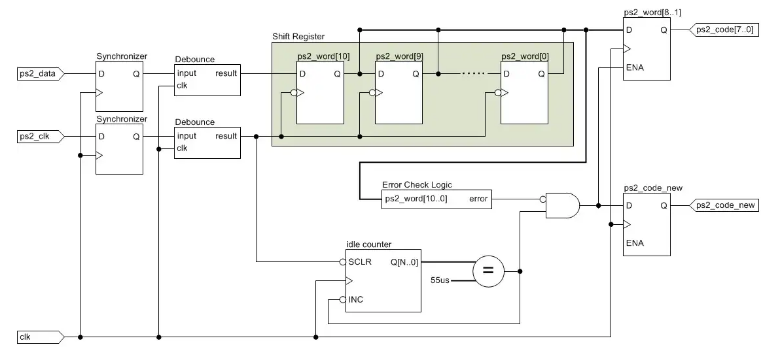
\includegraphics[width=.8\textwidth]{functional_units/ps2_keyboard/ps2_keyboard_block.png}
\caption{The logic design of the ps2\_keyboard functional unit used in the final design.}
\end{figure}
\begin{figure}[h]
\centering
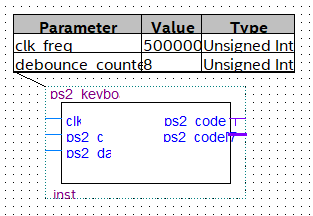
\includegraphics[width=.48\textwidth]{functional_units/ps2_keyboard/ps2_keyboard_symbol.png}
\caption{The block symbol of the ps2\_keyboard functional unit used in the final design.}
\end{figure}
\begin{figure}[h]
\centering
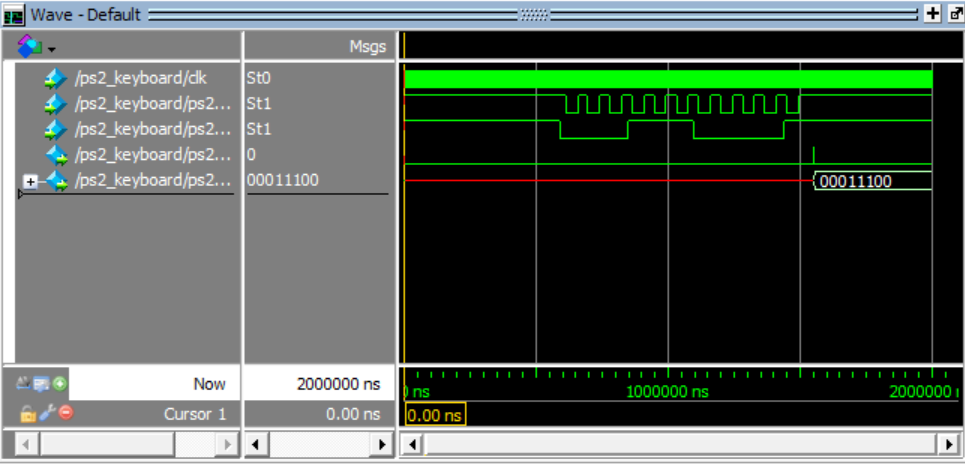
\includegraphics[width=.98\textwidth]{functional_units/ps2_keyboard/ps2_keyboard_sim.png}
\caption{The simulation results for the ps2\_keyboard module.}
\end{figure}
\clearpage

\catcode`\_=13
\def_{\textunderscore}
\subsubsection{debounce Component Block}
\catcode`_=8
When using mechanical switches, the signals often rebound, or bounce, off one another before settling into a stable state. The debounce component is used for successfully sending the data in a stable state. Two flip flops in the design check whether the data changes or not via the XOR gate. If the data changes, the counter block receives the signal to reset the counter. If not, the counter increases until it reaches the specified time and enables the output register. According to simulation, when the data remains stable for 40 ns, the data is sent to the last flip flop and the result signal is updated.  A block diagram follows in 	extbf{Figure 35}.  The simulation results follow in \textbf{Figure 36}.
\begin{itemize}
\item \textbf{Inputs:  } The debounce block has one input: button. It indicates the input from the keyboard.
\item \textbf{Outputs: } The debounce block has one output: result. It has the debounced value of the button.
\end{itemize}
\begin{figure}[h]
\centering
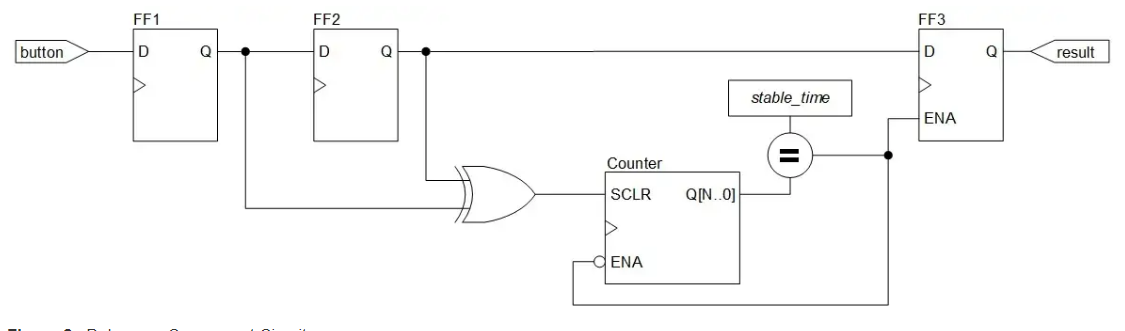
\includegraphics[width=.8\textwidth]{functional_units/ps2_keyboard/individual_blocks/debounce_block.png}
\caption{The logic design of the debounce module used in the ps2\_keyboard functional unit.}
\end{figure}
\begin{figure}[h]
\centering
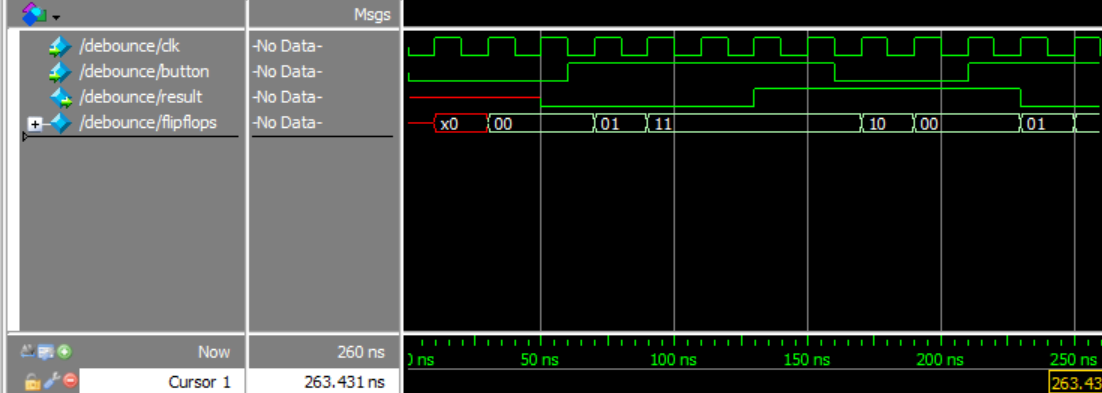
\includegraphics[width=.98\textwidth]{functional_units/ps2_keyboard/individual_blocks/debounce_sim.png}
\caption{The simulation results for the debounce module used in the ps2\_keyboard functional unit.}
\end{figure}
\clearpage

\catcode`\_=13
\def_{\textunderscore}
\subsection{nes\_decoder Functional Unit}
\catcode`_=8
The nes\_decoder module interfaces with inputs from and outputs to the nes controller hardware to parse the states (active low) of the eight buttons on the controller. The logic symbol follows in \textbf{Figure 37}.  The simulation results follow in \textbf{Figure 38}.
\begin{itemize}
\item \textbf{Inputs:  } An input clock (at 50MHz for this design) which determines how quickly the system reads the nes inputs; an nes\_data input that is the serialized data from the nes controller which describes the buttons pushed at any given moment; a reset signal that sets the system back to a default state; and a read\_data input that, when driven high while the system is ready to read, starts the reading process. The nes\_data input is the only input connected to the nes controller.
\item \textbf{Outputs: } Two outputs (nes\_latch and nes\_clock) that are sent to the nes controller and signal to the controller to start sending the first or next button states along nes\_data, respectively; ready\_to\_read, which is driven high by the module after the system has completed an input reading period and is ready for another round of reading; and eight outputs describing the most recently read states of each of the buttons on the nes controller (active low, they are the A, B, Start, Select, Up, Down, Left, and Right Buttons).
\end{itemize}
\begin{figure}[h]
\centering
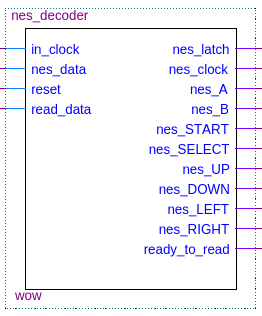
\includegraphics[width=.48\textwidth]{functional_units/nes_decoder/nes_decoder_symbol.png}
\caption{The block symbol of the nes\_decoder functional unit used in the final design.}
\end{figure}
\begin{figure}[h]
\centering
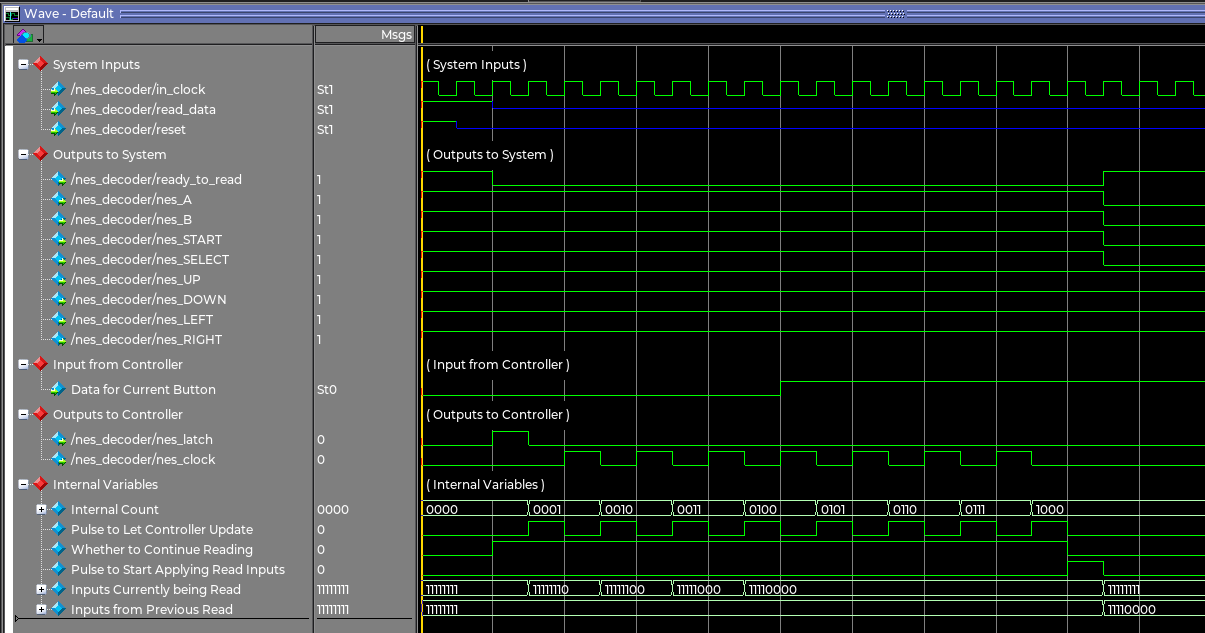
\includegraphics[width=.98\textwidth]{functional_units/nes_decoder/nes_decoder_sim.png}
\caption{The simulation results for the nes\_decoder module.}
\end{figure}
\clearpage

\catcode`\_=13
\def_{\textunderscore}
\subsection{parsed\_clock Functional Unit}
\catcode`_=8
The parsed\_clock module takes in a clock and some control signals that start, modify the speed of, and reset a clock that is accurate to 1Hz. These outputs are parsed into seconds, minutes, and hours (in decimal notation) to match the typcial clock format of (HH.MM.SS). The inputs come from the nes\_decoder and the FPGA's internal pins, and the outputs all go to the seven\_seg\_6 (six-digit seven segment display decoder) module in the design. A block diagram follows in \textbf{Figure 39}.  The logic symbol follows in \textbf{Figure 40}.  The simulation results follow in \textbf{Figure 41}.
\begin{itemize}
\item \textbf{Inputs:  } A 50Mhz clock from the FPGA's internal pins; a reset signal from either the active-high button state of the B button on the nes controller or the overall system\_reset signal that is the active-high button state of a button on the FPGA itself; and four more active-high button states from the nes controller (A Button acting as the start (toggle) enable signal of the clock, Start Button acting as the double-speed mode input of the parsed clock while held, and the Select Button acting as the super-speed mode input of the parsed clock while held).
\item \textbf{Outputs: } Six 4-bit binary value outputs describing the one's and ten's places of the seconds, minutes, and hours of the parsed clock. These values never exceed 59 seconds, 59 minutes, and 23 hours, so overflow is impossible. These outputs all directly lead to the seven\_seg\_6 module that converts these 4-bit values into seven segment endcoded values.
\end{itemize}
\begin{figure}[h]
\centering
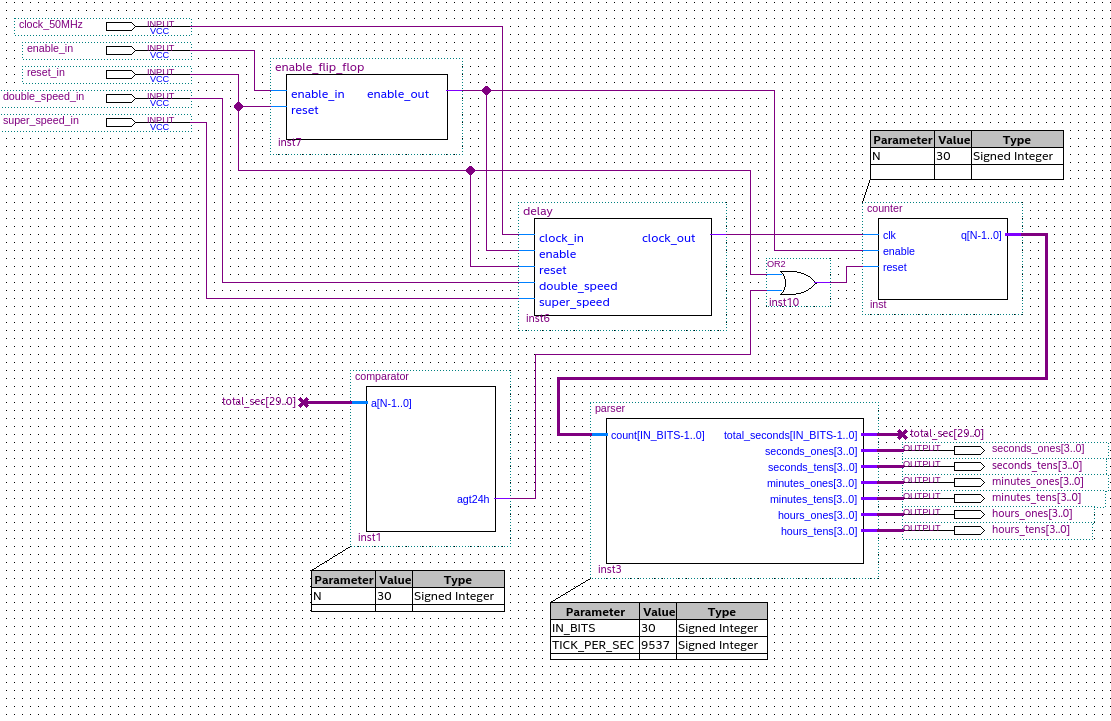
\includegraphics[width=.8\textwidth]{functional_units/parsed_clock/parsed_clock_block.png}
\caption{The logic design of the parsed\_clock functional unit used in the final design.}
\end{figure}
\begin{figure}[h]
\centering
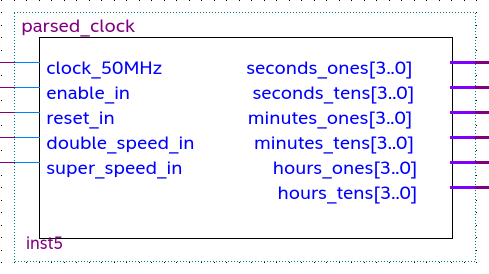
\includegraphics[width=.48\textwidth]{functional_units/parsed_clock/parsed_clock_symbol.png}
\caption{The block symbol of the parsed\_clock functional unit used in the final design.}
\end{figure}
\begin{figure}[h]
\centering
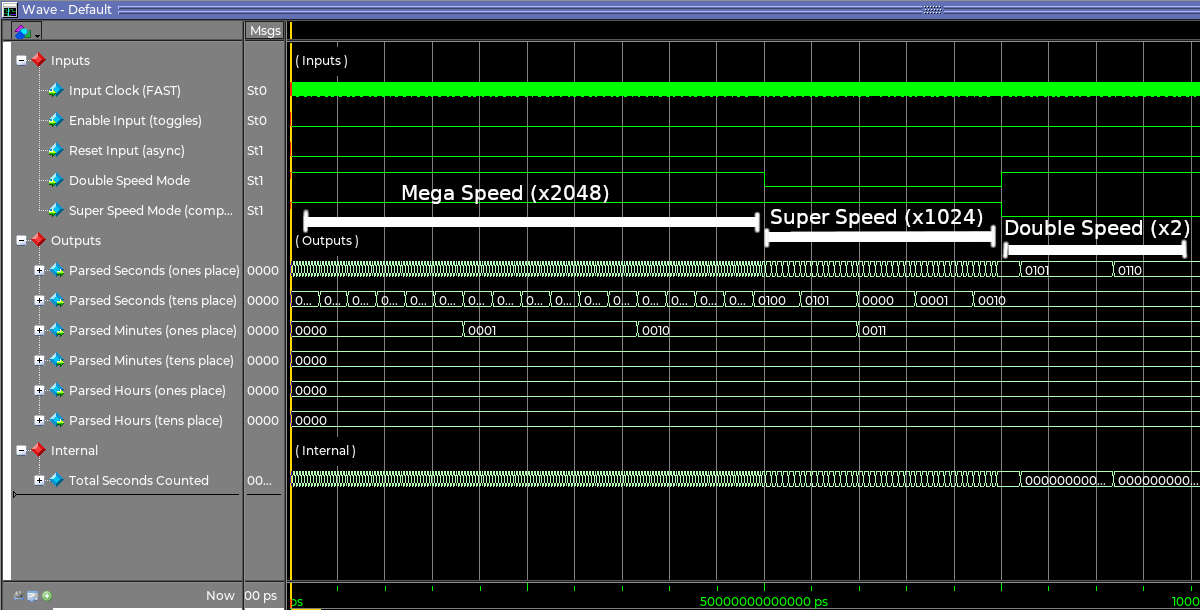
\includegraphics[width=.98\textwidth]{functional_units/parsed_clock/parsed_clock_sim.png}
\caption{The simulation results for the parsed\_clock module.}
\end{figure}
\clearpage

\catcode`\_=13
\def_{\textunderscore}
\subsubsection{enable\_flip\_flop Component Block}
\catcode`_=8
The enable\_flip\_flop submodule acts to toggle whether the clock is enabled (should count). It does this by taking in an enable input from the design, and on the positive edge of this enable, toggling it's enable\_out output. It can be reset. The logic symbol follows in \textbf{Figure 42}.  The simulation results follow in \textbf{Figure 43}.
\begin{itemize}
\item \textbf{Inputs:  } An input enable\_in that, on its rising edge, toggles the outputted enable value of the module; and a reset input that resets the flip\_flop to logic low.
\item \textbf{Outputs: } An output that represents whether the clock should count or not (the submodule's enable value). This goes to the delay and counter blocks.
\end{itemize}
\begin{figure}[h]
\centering
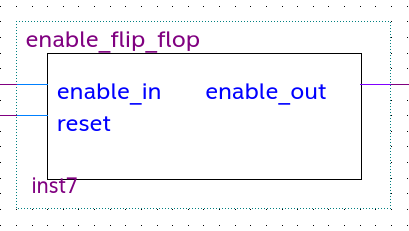
\includegraphics[width=.48\textwidth]{functional_units/parsed_clock/individual_blocks/enable_flip_flop_symbol.png}
\caption{The block symbol of the enable\_flip\_flop module used in the parsed\_clock functional unit.}
\end{figure}
\begin{figure}[h]
\centering
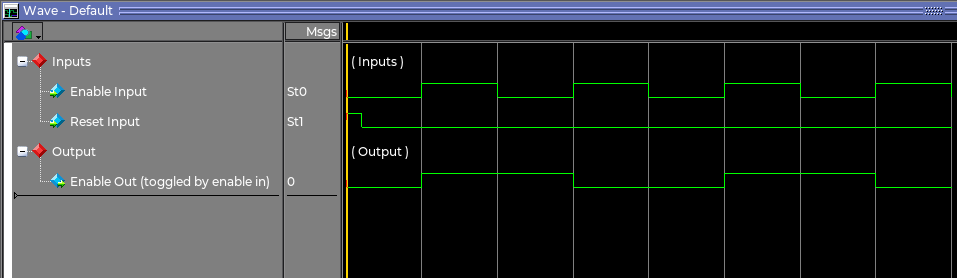
\includegraphics[width=.98\textwidth]{functional_units/parsed_clock/individual_blocks/enable_flip_flop_sim.png}
\caption{The simulation results for the enable\_flip\_flop module used in the parsed\_clock functional unit.}
\end{figure}
\clearpage

\catcode`\_=13
\def_{\textunderscore}
\subsubsection{delay Component Block}
\catcode`_=8
The delay submodule, by default, slows an input clock down by a factor of 1/2 to the 10. This is so that an input clock of 50MHz (as in this design) is slowed to a frequency that is easier converted to 1Hz later on through division. This submodule also allows for 4 modes of speed (MEGA, Super, Double, and Normal speeds). MEGA is 2048, Super is 1024, and Double is 2 times as fast as the Normal speed. This is controlled by the values of two speed inputs that act as a select signal between these options. A block diagram follows in 	extbf{Figure 44}.  The logic symbol follows in \textbf{Figure 45}.  The simulation results follow in \textbf{Figure 46}.
\begin{itemize}
\item \textbf{Inputs:  } An input clock to be slowed (50Mhz in this design); an active-high enable that allows the submodule to propagate signal; a reset signal to reset all flip\_flops to 1 (such that the first signal overflows and sends all held values to 0); and two inputs (double\_speed and super\_speed) that combine as a select signal to choose between four possible output clock speeds (MEGA 1,1 , Super 1,0 , Double 0,1 , and Normal 0,0 speeds for the select signal super\_speed, double\_speed).
\item \textbf{Outputs: } A clock that is 1/2 to the 10 slower than the input clock in normal mode, somewhat faster depending on the speed mode selected (described above).
\end{itemize}
\begin{figure}[h]
\centering
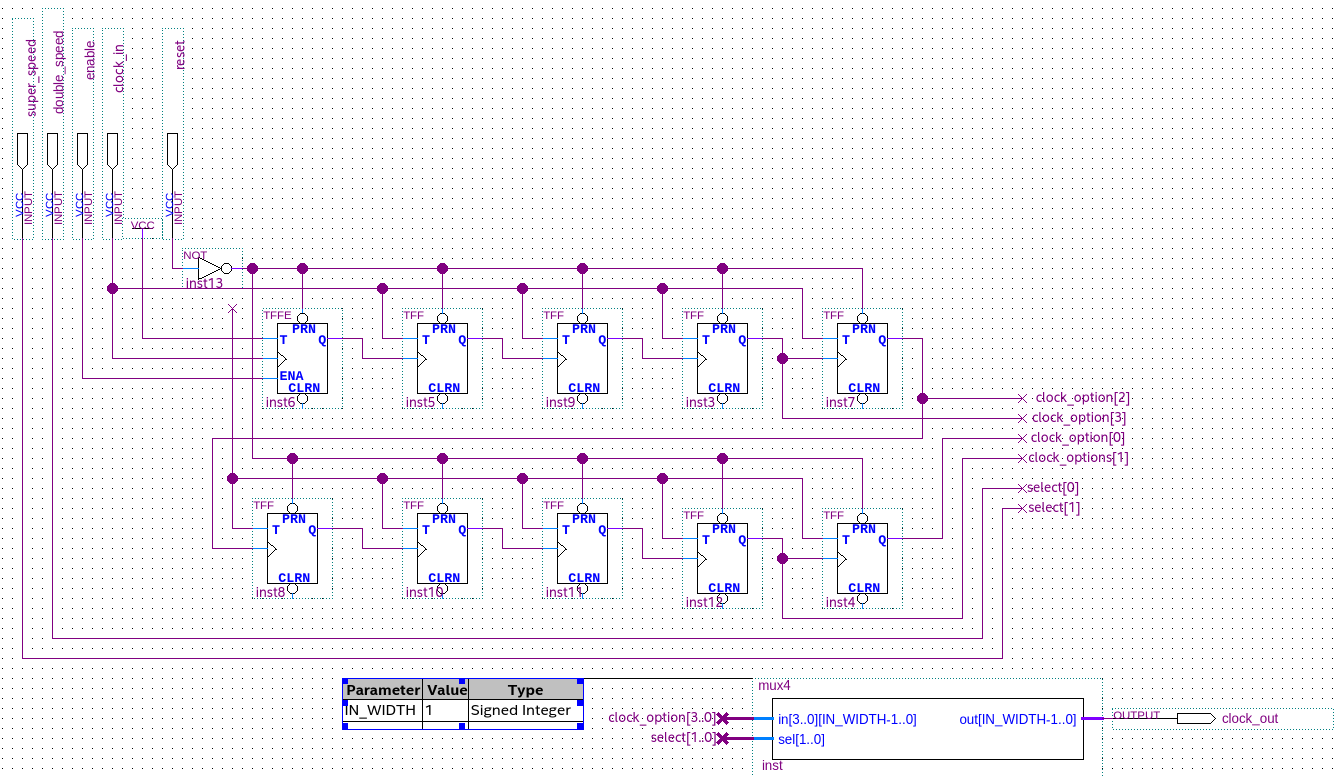
\includegraphics[width=.8\textwidth]{functional_units/parsed_clock/individual_blocks/delay_block.png}
\caption{The logic design of the delay module used in the parsed\_clock functional unit.}
\end{figure}
\begin{figure}[h]
\centering
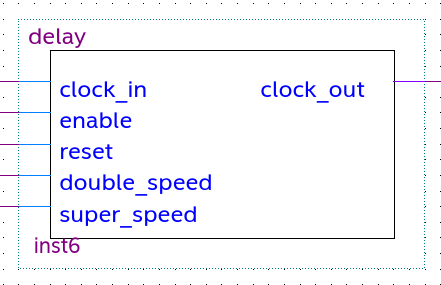
\includegraphics[width=.48\textwidth]{functional_units/parsed_clock/individual_blocks/delay_symbol.png}
\caption{The block symbol of the delay module used in the parsed\_clock functional unit.}
\end{figure}
\begin{figure}[h]
\centering
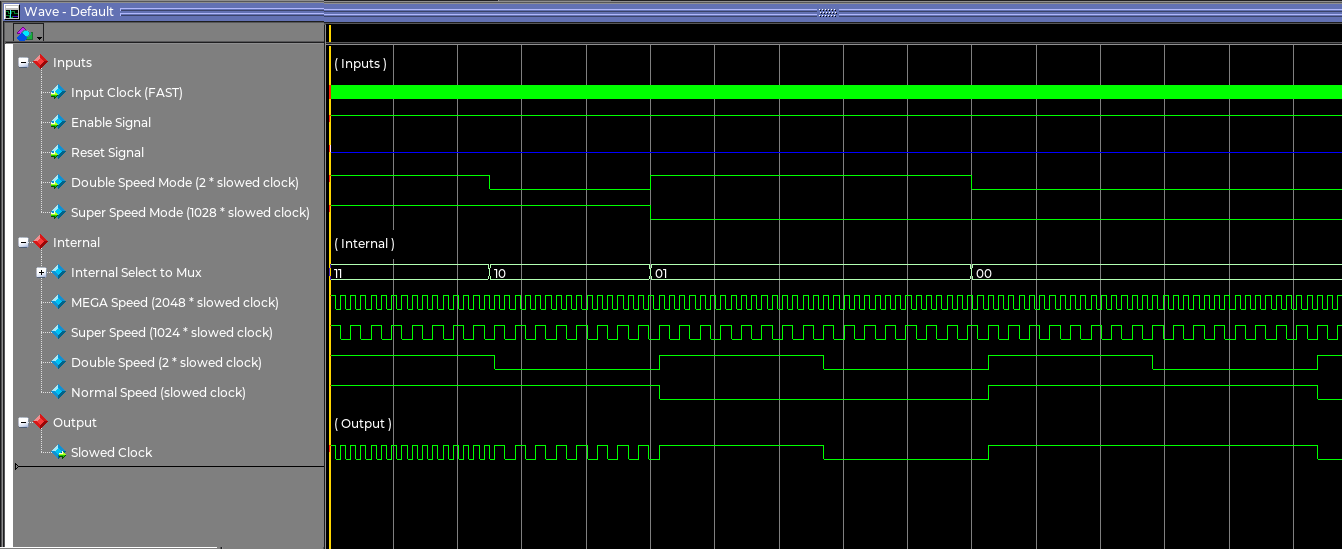
\includegraphics[width=.98\textwidth]{functional_units/parsed_clock/individual_blocks/delay_sim.png}
\caption{The simulation results for the delay module used in the parsed\_clock functional unit.}
\end{figure}
\clearpage

\catcode`\_=13
\def_{\textunderscore}
\subsubsection{mux4 Component Block}
\catcode`_=8
The mux4 submodule is a 4-option mux (where each option in this design is a one-wide clock speed option). This accounts for the select signals in the delay block. The logic symbol follows in \textbf{Figure 47}.  The simulation results follow in \textbf{Figure 48}.
\begin{itemize}
\item \textbf{Inputs:  } Four one-bit options to send to the output (the speed options of the delay block); and a 2-bit select signal that maps select values 11, 10, 01, and 00 to sending clock\_options 3, 2, 1, and 0.
\item \textbf{Outputs: } One 1-bit output from the 4 options presented in the inputs, selected by the select signal. This is also the output of the delay block.
\end{itemize}
\begin{figure}[h]
\centering
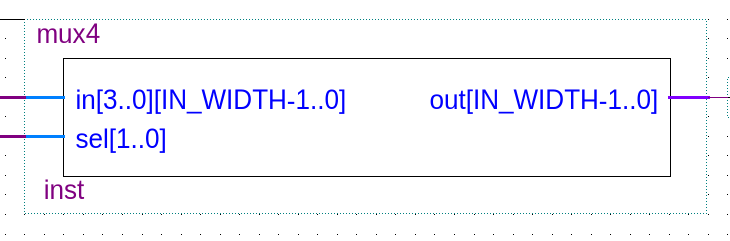
\includegraphics[width=.48\textwidth]{functional_units/parsed_clock/individual_blocks/mux4_symbol.png}
\caption{The block symbol of the mux4 module used in the parsed\_clock functional unit.}
\end{figure}
\begin{figure}[h]
\centering
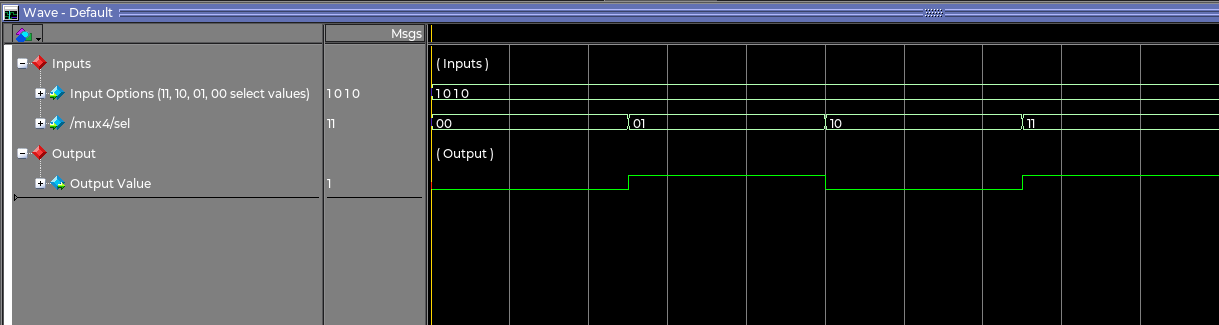
\includegraphics[width=.98\textwidth]{functional_units/parsed_clock/individual_blocks/mux4_sim.png}
\caption{The simulation results for the mux4 module used in the parsed\_clock functional unit.}
\end{figure}
\clearpage

\catcode`\_=13
\def_{\textunderscore}
\subsubsection{counter Component Block}
\catcode`_=8
The counter submodule is a simple one-by counter that increments it's output q on every clock cycle. It has a default max width of q of 30-bits and can be reset and enabled via its inputs. The logic symbol follows in \textbf{Figure 49}.  The simulation results follow in \textbf{Figure 50}.
\begin{itemize}
\item \textbf{Inputs:  } A clock signal (clk) on which to increment the count held in the q output; a reset signal which sets the q output back to 0; and an enable signal that determines whether the counter should react to the clock.
\item \textbf{Outputs: } The count output held in the output q, with a default maximum width of 30-bits.
\end{itemize}
\begin{figure}[h]
\centering
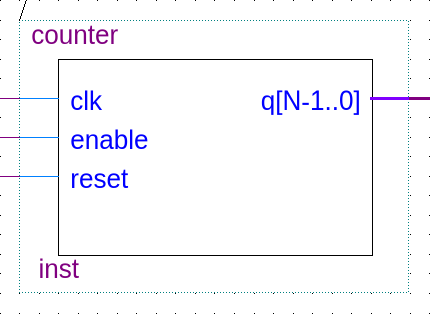
\includegraphics[width=.48\textwidth]{functional_units/parsed_clock/individual_blocks/counter_symbol.png}
\caption{The block symbol of the counter module used in the parsed\_clock functional unit.}
\end{figure}
\begin{figure}[h]
\centering
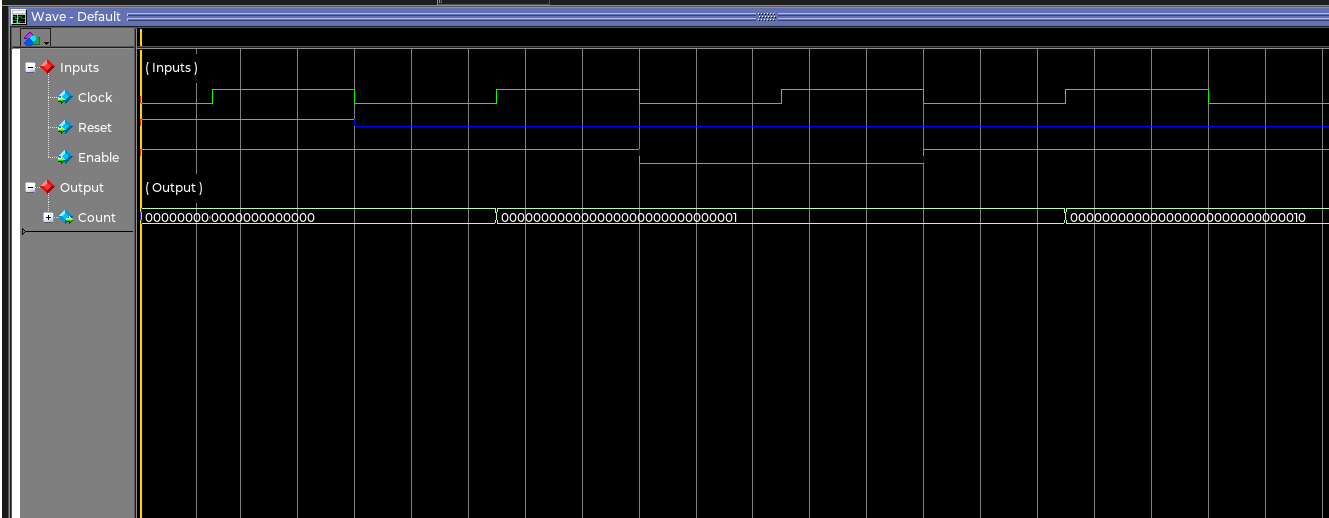
\includegraphics[width=.98\textwidth]{functional_units/parsed_clock/individual_blocks/counter_sim.png}
\caption{The simulation results for the counter module used in the parsed\_clock functional unit.}
\end{figure}
\clearpage

\catcode`\_=13
\def_{\textunderscore}
\subsubsection{parser Component Block}
\catcode`_=8
The parser submodule takes in a binary value up to 30-bits wide of slowed clock ticks, divides it by the number of clock ticks per second (9537 in this design, due to the delay block), and parses it into seconds, minutes, and hours (in decimal notation) to match the typcial clock format of (HH.MM.SS). The logic symbol follows in \textbf{Figure 51}.  The simulation results follow in \textbf{Figure 52}.
\begin{itemize}
\item \textbf{Inputs:  } The count of clock ticks of the parsed\_clock module, outputted by the counter submodule.
\item \textbf{Outputs: } The total seconds counted so far (used for resetting at 24 hours), and six 4-bit binary value outputs describing the one's and ten's places of the seconds, minutes, and hours of the parsed clock.
\end{itemize}
\begin{figure}[h]
\centering
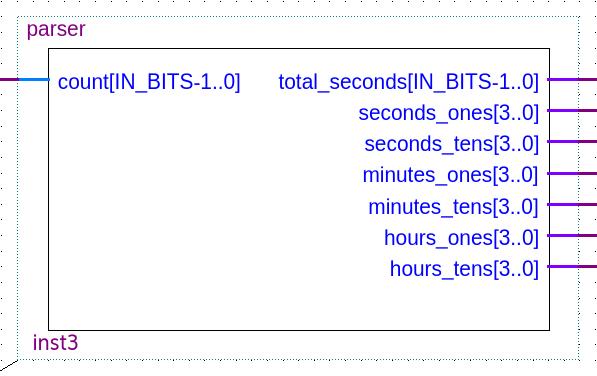
\includegraphics[width=.48\textwidth]{functional_units/parsed_clock/individual_blocks/parser_symbol.png}
\caption{The block symbol of the parser module used in the parsed\_clock functional unit.}
\end{figure}
\begin{figure}[h]
\centering
\includegraphics[width=.98\textwidth]{functional_units/parsed_clock/individual_blocks/parser_sim.png}
\caption{The simulation results for the parser module used in the parsed\_clock functional unit.}
\end{figure}
\clearpage

\catcode`\_=13
\def_{\textunderscore}
\subsubsection{comparator Component Block}
\catcode`_=8
The comparator submodule takes in the total seconds counted by the parsed clock since the last reset, and sends a signal to reset the system when it is greater than or equal to the number of seconds in 24 hours. This prevents the clock from outputting values over what is possible in the typical clock format (HH.MM.SS). The logic symbol follows in \textbf{Figure 53}.  The simulation results follow in \textbf{Figure 54}.
\begin{itemize}
\item \textbf{Inputs:  } The total seconds counted by the parsed clock since the last reset (default max width of 30-bits, called a).
\item \textbf{Outputs: } Whether the total seconds input (a) is greater than or equal to the number of seconds in a day ($60*60*24=3600$).
\end{itemize}
\begin{figure}[h]
\centering
\includegraphics[width=.48\textwidth]{functional_units/parsed_clock/individual_blocks/comparator_symbol.png}
\caption{The block symbol of the comparator module used in the parsed\_clock functional unit.}
\end{figure}
\begin{figure}[h]
\centering
\includegraphics[width=.98\textwidth]{functional_units/parsed_clock/individual_blocks/comparator_sim.png}
\caption{The simulation results for the comparator module used in the parsed\_clock functional unit.}
\end{figure}
\clearpage

\catcode`\_=13
\def_{\textunderscore}
\subsection{SquareWaveGenerator Functional Unit}
\catcode`_=8
Square Wave Generator generates square wave and it is used to generate tones in the piano in this project. When ps2\_code[7..0] is read from the PS/2 Keyboard functional unit, a decoder decodes the data into three-digit binary data. The SquareWaveGenerator block receives the data and converts it into the square wave with specific Hz that indicates notes in the piano.
\begin{itemize}
\item \textbf{Inputs:  } The square wave generator schematic has three inputs, clk\_50MHz, ps2\_code[7..0], en. The clk\_50MHz is the clock with a frequency of 50MHz, ps2\_code[7..0] is the 8-bit data sent from PS/2 keyboard, and en is the switch that allows the SquareWaveGenerator block to send a data to output signal sqWave.
\item \textbf{Outputs: } The square wave generator schematic has one output, sqWave. It shows the square wave with a specific Hz to generate the tone in the piano.
\end{itemize}
\clearpage

\catcode`\_=13
\def_{\textunderscore}
\subsubsection{SquareWaveGenerator Component Block}
\catcode`_=8
The square wave generator block converts eight types of 3-bit data from 0b000 to 0b111 into a square wave. In the SystemVerilog file, the internal counter div\_cnt is compared to max\_count which indicates the period taken to reach specific hz. If div\_cnt reaches max\_count, tmp\_clk changes to make a square wave. The en signal determines whether the tmp\_clk is sent to speaker or not. To make it clear, max\_count for middle C is 95419 because the period for 262Hz is 3816973ns. Considering that the clock has the frequency of 50MHz, the signal is read in every 20ns and the square wave should be changed after it passes half of the period. Therefore, after calculating 3816973/20/2=95419. The max\_count for other notes is also derived from this calculation. The notes from the middle C to the C with next octave have the frequency of 262 Hz, 294 Hz, 330 Hz, 350 Hz, 392 Hz, 440 Hz, 494 Hz, and 523 Hz in sequence. This means that each note has the period of 381673 ns, 3401360 ns, 3030303 ns, 2857142 ns, 2551020 ns, 2272727 ns, 2024291 ns, and 1912045 ns respectively. When they are simulated in the period, the square wave changes only once at the half of the period as shown below. The logic symbol follows in \textbf{Figure 55}.  The simulation results follow in \textbf{Figure 56}.
\begin{itemize}
\item \textbf{Inputs:  } The SquareWaveGenerator block has four inputs, clk, note[2..0], en, and reset. The clk is the clock with a frequency of 50MHz, and note[2..0] is the decoded data from the decoder to determine the note to generate. The en and reset performs as a switch for the block.
\item \textbf{Outputs: } The SquareWaveGenerator block has one input, speaker. It shows the square wave generated from the block.
\end{itemize}
\begin{figure}[h]
\centering
\includegraphics[width=.48\textwidth]{functional_units/SquareWaveGenerator/individual_blocks/SquareWaveGenerator_symbol.png}
\caption{The block symbol of the SquareWaveGenerator module used in the SquareWaveGenerator functional unit.}
\end{figure}
\begin{figure}[h]
\centering
\includegraphics[width=.98\textwidth]{functional_units/SquareWaveGenerator/individual_blocks/SquareWaveGenerator_sim.png}
\caption{The simulation results for the SquareWaveGenerator module used in the SquareWaveGenerator functional unit.}
\end{figure}
\clearpage

\catcode`\_=13
\def_{\textunderscore}
\subsubsection{decoder Component Block}
\catcode`_=8
The decoder block decodes the data from the PS/2 keyboard to the three-bit data. To match the keys in keyboard from a to t with the piano notes from middle C to the upper octave C, the hexadecimal code of the keyboard is converted to 3-bit data as shown in the simulation.  The logic symbol follows in \textbf{Figure 57}.  The simulation results follow in \textbf{Figure 58}.
\begin{itemize}
\item \textbf{Inputs:  } The decoder block has one input, a[7..0]. It indicates the input 8-bit data, which is the make code for keys on the keyboard.
\item \textbf{Outputs: } The decoder block has one input, y[2..0]. It is converted from 8-bit to 3-bit data and is used to determine the note to generate.
\end{itemize}
\begin{figure}[h]
\centering
\includegraphics[width=.48\textwidth]{functional_units/SquareWaveGenerator/individual_blocks/decoder_symbol.png}
\caption{The block symbol of the decoder module used in the SquareWaveGenerator functional unit.}
\end{figure}
\begin{figure}[h]
\centering
\includegraphics[width=.98\textwidth]{functional_units/SquareWaveGenerator/individual_blocks/decoder_sim.png}
\caption{The simulation results for the decoder module used in the SquareWaveGenerator functional unit.}
\end{figure}
\clearpage

\catcode`\_=13
\def_{\textunderscore}
\subsection{nes\_to\_motor Functional Unit}
\catcode`_=8
The nes\_to\_motor module converts nes button states coming from the nes\_deccoder module and converts them to the signals used internally in the L293D\_encoder module to interface with the L293D DC motor controller. This is a module completely internal to the design that converts between the output and input signal conventions of other modules. The logic symbol follows in \textbf{Figure 59}.  The simulation results follow in \textbf{Figure 60}.
\begin{itemize}
\item \textbf{Inputs:  } Four active-high inputs describing that a system of two motors (like a tank) should turn left (left), turn right (right), drive forward (forward), or drive backward (backward), respectively. In this design, these inputs come from the inverted left, right, up, and down button states of the nes controller.
\item \textbf{Outputs: } Whether motors 1 (left) and 2 (right) should be spinning (motor\_1\_on and motor\_2\_on); and which direction each motor should spin if also enabled, where logic high correlates to clockwise motion and low to counterclockwise (motor\_1\_dir and motor\_2\_dir for each motor, respectively).
\end{itemize}
\begin{figure}[h]
\centering
\includegraphics[width=.48\textwidth]{functional_units/nes_to_motor/nes_to_motor_symbol.png}
\caption{The block symbol of the nes\_to\_motor functional unit used in the final design.}
\end{figure}
\begin{figure}[h]
\centering
\includegraphics[width=.98\textwidth]{functional_units/nes_to_motor/nes_to_motor_sim.png}
\caption{The simulation results for the nes\_to\_motor module.}
\end{figure}
\clearpage

\catcode`\_=13
\def_{\textunderscore}
\subsection{Comparator Functional Unit}
\catcode`_=8
The Comparator Functional Unit is used to create a clock that operates at 10 KHz, to drive the vcr\_decoder Functional Unit. The FPGA clock is 50 MHz so in order to create a 10 KHz clock, we only want a rising edge every 5000 cycles of the FPGA clock.  The logic symbol follows in \textbf{Figure 61}.  The simulation results follow in \textbf{Figure 62}.
\begin{itemize}
\item \textbf{Inputs:  } The Comparator Functional Unit has a single input: a. a is a 23-bit value that is the output of the Counter Functional Unit
\item \textbf{Outputs: } The Comparator Functional Unit has a single output: eq. eq is one if the input value, a, is equal to 5000.
\end{itemize}
\begin{figure}[h]
\centering
\includegraphics[width=.48\textwidth]{functional_units/Comparator/Comparator_symbol.png}
\caption{The block symbol of the Comparator functional unit used in the final design.}
\end{figure}
\begin{figure}[h]
\centering
\includegraphics[width=.98\textwidth]{functional_units/Comparator/Comparator_sim.png}
\caption{The simulation results for the Comparator module.}
\end{figure}
\clearpage

\catcode`\_=13
\def_{\textunderscore}
\subsection{DisplayDecoder Functional Unit}
\catcode`_=8
The DisplayDecoder Module converts a 4-bit input value into a display value on the seven segment display of the FPGA. The DisplayDecoder is able to output a hexadecimal display value between 0 and F.
\begin{itemize}
\item \textbf{Inputs:  } The DisplayDecoder module takes a 4-bit binary value input, data, as its only input.
\item \textbf{Outputs: } The DisplayDecoder module outputs a 7-bit binary value that is used to activate specific segments in the FPGA seven segment display.
\end{itemize}
\clearpage








\clearpage



\subsection{DisplaysDecoder Functional Unit}
The DisplayDecoder Module converts a 4-bit input value into a display value on the seven segment display of the FPGA. The DisplayDecoder is
able to output a hexadecimal display value between 0 and F. A block diagram of the unit follows in \textbf{Figure A} and the simulation results for the unit follows in \textbf{Figure B}.
\begin{itemize}
  \item \textbf{Inputs:  } The DisplayDecoder module takes a 4-bit binary value input, data, as its only input.
  \item \textbf{Outputs: } The DisplayDecoder module outputs a 7-bit binary value that is used to activate specific segments in the FPGA seven segment display.
\end{itemize}
\begin{figure}[h]
  \centering
    \includegraphics[width=.8\textwidth]{images/functional_1.png}
	\caption{The logic design of the DisplayDecoder functional unit used in the final design.}
    \label{fig:functional-1}
\end{figure}
\begin{figure}[h]
  \centering
    \includegraphics[width=.98\textwidth]{sims/functional_1.png}
	\caption{The simulation results for the DisplayDecoder Individual Unit.}
    \label{fig:top-level-sim}
\end{figure}



\clearpage



\subsection{vcr\_decoder Functional Unit}
The vcr\_decoder module converts an IR signal sent from a VCR remote into a decimal value between 0 and 9. A block diagram of the unit follows in \textbf{Figure A}. A state diagram describing the unit as well as the simulation results for the unit follow in \textbf{Figure B}, and the details for each individual block comprising the unit follow after.
\subsection{vcr decoder Functional Unit}
The vcr\_decoder module converts an IR signal sent from a VCR remote into a decimal value between 0 and 9. A block diagram of the unit follows in \textbf{Figure A}, the simulation results for the unit follows in \textbf{Figure B}, and the details for each individual block comprising the unit follow after.
\begin{itemize}
  \item \textbf{Inputs:  } The vcr\_decoder module two inputs, clk and IR. clk is a 10 KHz clock signal that is used to drive the module. IR is the Infrared signal coming from the VCR remote that will be translated by the module.
  \item \textbf{Outputs: } The vcr\_decoder module has a single output, displayValue, which is the 0-9 representing the IR signal that was received by the module as input.
\end{itemize}
\begin{figure}[h]
  \centering
    \includegraphics[width=.8\textwidth]{images/functional_1.png}
	\caption{The logic design of the vcr\_decoder functional unit used in the final design.}
    \label{fig:functional-1}
\end{figure}
\begin{figure}[h]
  \centering
    \includegraphics[width=.8\textwidth]{images/functional_1.png}
	\caption{The State Diagram for the vcr\_decoder functional unit used in the final design.}
    \label{fig:functional-1}
\end{figure}
\begin{figure}[h]
  \centering
    \includegraphics[width=.98\textwidth]{sims/vcr_testing/moduleTests/vcr_decoder/IDLE_to_C1_Transition.png}
	\caption{Simulation results of the vcr\_decoder Functional Unit showing the state transition from the IDLE state to the C1 control state following the first time the IR signal goes to a logic LOW.}
    \label{fig:top-level-sim}
\end{figure}
\begin{figure}[h]
  \centering
    \includegraphics[width=.98\textwidth]{sims/vcr_testing/moduleTests/vcr_decoder/C1_to_C2_transition.png}
	\caption{Simulation results of the vcr\_decoder Functional Unit showing the state transition from the C1 control state to the C2 control state.}
    \label{fig:top-level-sim}
\end{figure}
\begin{figure}[h]
  \centering
    \includegraphics[width=.98\textwidth]{sims/vcr_testing/moduleTests/vcr_decoder/C2_to_READ_transition.png}
	\caption{Simulation results of the vcr\_decoder Functional Unit showing the transition from the C2 control state to the READ state, indicicating that it is currently reading a 32-bit IR signal corresponding the button on the VCR remote that was pressed.}
    \label{fig:top-level-sim}
\end{figure}
\begin{figure}[h]
  \centering
    \includegraphics[width=.98\textwidth]{sims/vcr_testing/moduleTests/vcr_decoder/READ_to_PUSH_transition.png}
	\caption{Simulation results of the vcr\_decoder Functional Unit showing the transition from the READ state to the PUSH state indicating that the full 32-bit input value has been processed and an output value is produced.}
    \label{fig:top-level-sim}
\end{figure}




\clearpage



\subsubsection{ReadState Individual Block}
The ReadState Individual Block is used to implement the READ state within the vcr\_decoder Module. The block diagram (\textbf{Figure C}), State Diagram, and simulation results \textbf{Figure D} are provided below.
\begin{itemize}
  \item \textbf{Inputs:  } inputs
  \item \textbf{Outputs: } outputs
\end{itemize}
\begin{figure}[h]
  \centering
  \includegraphics[width=.48\textwidth]{symbols/individual_placeholder.png}
  \caption{The block symbol of the ReadState individual block used in the vcr\_decoder functional unit.}
    \label{fig:individual-1-2-block}
\end{figure}
\begin{figure}[h]
  \centering
  \includegraphics[width=.98\textwidth]{sims/vcr_testing/moduleTests/ReadState/IDLE_to_READING_Transition.png}
  \caption{Simulation results of the ReadState individual block used in the vcr\_decoder functional unit. The simulation shows the transition from the IDLE state to the Reading State within the ReadState Module. This transition is in response to the initial HIGH IR signal that represents the 32-bit value encoding the button that was pressed.}
    \label{fig:individual-1-2-sim}
\end{figure}
\begin{figure}[h]
  \centering
  \includegraphics[width=.98\textwidth]{sims/vcr_testing/moduleTests/ReadState/PROCESSING_State.png}
  \caption{Simulation results of the ReadState individual block used in the vcr\_decoder functional unit. The simulation shows Processing State of the ReadState Module. When the state machine is in the Reading state, that means it is actively reading a HIGH signal for IR. As seen in this waveform, when IR goes LOW again, the state machine switches to the Processing state in which it checks the length of the signal to see if it is a logic 1 or a logic 0. The 1 or 0 is then shifted into the shift register on the rising edge of the shiftValue signal, as seen in the waveform. The state machine then switches into the Waiting state, while it waits for IR to go HIGH again.}
    \label{fig:individual-1-2-sim}
\end{figure}
\begin{figure}[h]
  \centering
  \includegraphics[width=.98\textwidth]{sims/vcr_testing/moduleTests/ReadState/Transition_to_DONE.png}
  \caption{Simulation results of the ReadState individual block used in the vcr\_decoder functional unit. The simulation shows the transition from the reading, Processing, Waiting cycle to the Done state in which it outputs the 32-bit hexadecimal value identified by the IR signal input. In each Waiting state, the state machine will check if 32-bits have been read into the shift register. If so, the state machine will switch to the Done state and output the value for the IR signal that it received as input. In addition, it will drive an output signal outputReady HIGH. This signal is used by the vcr\_decoder module, to know when to output a result.}
    \label{fig:individual-1-2-sim}
\end{figure}



\clearpage



\subsubsection{SignalDecoder Individual Block}
The SignalDecoder Individual Block is used to convert the 32-bit value generated by the ReadState Individual Block into a 4-bit value by 0 and 15 that indicated which button on the VCR remote was pressed. The input and output specifications follow, as well as the block diagram (\textbf{Figure C}), and simulation results \textbf{Figure D} for the individual block.
\begin{itemize}
  \item \textbf{Inputs:  } The SignalDecoder Individual Block takes a single 32-bit input that corresponds to the complete IR signal that was read in by the ReadState Individual Block
  \item \textbf{Outputs: } The SignalDecoder Individual Block outputs a 4-bit value betwee 0 and 15.
\end{itemize}
\begin{figure}[h]
  \centering
  \includegraphics[width=.48\textwidth]{symbols/individual_placeholder.png}
  \caption{The block symbol of the (NAME) individual block used in the (NAME) functional unit.}
    \label{fig:individual-1-2-block}
\end{figure}
\begin{figure}[h]
  \centering
  \includegraphics[width=.98\textwidth]{sims/vcr_testing/moduleTests/SignalDecoder/SignalDecoder_sim.png}
  \caption{The simulation results of the SignalDecoder individual block used in the vcr\_decoder functional unit.}
    \label{fig:individual-1-2-sim}
\end{figure}



\clearpage



\subsubsection{ShiftRegister Individual Block}
The ShiftRegister Individual Block is used to store the 32-bit IR signal value bit by bit as as it is read in by the ReadState Module. The input and output specifications follow, as well as the block diagram (\textbf{Figure C}), and simulation results \textbf{Figure D} for the individual block.
\begin{itemize}
  \item \textbf{Inputs:  } Inputs
  \item \textbf{Outputs: } Output
\end{itemize}
\begin{figure}[h]
  \centering
  \includegraphics[width=.48\textwidth]{symbols/individual_placeholder.png}
  \caption{The block symbol of the ShiftRegister individual block used in the vcr\_decoder functional unit.}
    \label{fig:individual-1-2-block}
\end{figure}
\begin{figure}[h]
  \centering
  \includegraphics[width=.98\textwidth]{sims/vcr_testing/moduleTests/shiftRegister/ShiftRegister_sim.png}
  \caption{The simulation results of the ShiftRegister individual block used in the vcr\_decoder functional unit.}
    \label{fig:individual-1-2-sim}
\end{figure}



\clearpage



\appendix
\section{SystemVerilog Files}
This appendix will list the SystemVerilog code used for each block used in the design project.

\subsection{decoder}
decoder.sv
\lstinputlisting[style=verilog-style]{functional_units/decoder/decoder.sv}

\subsection{seven\_seg\_6}
\subsubsection{Component Blocks of seven\_seg\_6 Unit}
sevenseg.sv
\lstinputlisting[style=verilog-style]{functional_units/seven_seg_6/individual_blocks/sevenseg.sv}

\clearpage

\subsection{L293D\_encoder}
L293D\_encoder.sv
\lstinputlisting[style=verilog-style]{functional_units/L293D_encoder/L293D_encoder.sv}

\subsection{Counter}
Counter.sv
\lstinputlisting[style=verilog-style]{functional_units/Counter/Counter.sv}

\subsection{vga\_encoder}
\subsubsection{Component Blocks of vga\_encoder Unit}
vga\_640x480.sv
\lstinputlisting[style=verilog-style]{functional_units/vga_encoder/individual_blocks/vga_640x480.sv}

rgb\_decoder.sv
\lstinputlisting[style=verilog-style]{functional_units/vga_encoder/individual_blocks/rgb_decoder.sv}

clock\_modulator.sv
\lstinputlisting[style=verilog-style]{functional_units/vga_encoder/individual_blocks/clock_modulator.sv}

\clearpage

\subsection{vcr\_decoder}
vcr\_decoder.sv
\lstinputlisting[style=verilog-style]{functional_units/vcr_decoder/vcr_decoder.sv}

\subsubsection{Component Blocks of vcr\_decoder Unit}
ReadState.sv
\lstinputlisting[style=verilog-style]{functional_units/vcr_decoder/individual_blocks/ReadState.sv}

ShiftRegister.sv
\lstinputlisting[style=verilog-style]{functional_units/vcr_decoder/individual_blocks/ShiftRegister.sv}

mux2.sv
\lstinputlisting[style=verilog-style]{functional_units/vcr_decoder/individual_blocks/mux2.sv}

SignalDecoder.sv
\lstinputlisting[style=verilog-style]{functional_units/vcr_decoder/individual_blocks/SignalDecoder.sv}

\clearpage

\subsection{ps2\_keyboard}
ps2\_keyboard.sv
\lstinputlisting[style=verilog-style]{functional_units/ps2_keyboard/ps2_keyboard.sv}

\subsubsection{Component Blocks of ps2\_keyboard Unit}
debounce.sv
\lstinputlisting[style=verilog-style]{functional_units/ps2_keyboard/individual_blocks/debounce.sv}

\clearpage

\subsection{nes\_decoder}
nes\_decoder.sv
\lstinputlisting[style=verilog-style]{functional_units/nes_decoder/nes_decoder.sv}

\subsection{parsed\_clock}
\subsubsection{Component Blocks of parsed\_clock Unit}
parser.sv
\lstinputlisting[style=verilog-style]{functional_units/parsed_clock/individual_blocks/parser.sv}

comparator.sv
\lstinputlisting[style=verilog-style]{functional_units/parsed_clock/individual_blocks/comparator.sv}

mux4.sv
\lstinputlisting[style=verilog-style]{functional_units/parsed_clock/individual_blocks/mux4.sv}

counter.sv
\lstinputlisting[style=verilog-style]{functional_units/parsed_clock/individual_blocks/counter.sv}

\clearpage

\subsection{SquareWaveGenerator}
\subsubsection{Component Blocks of SquareWaveGenerator Unit}
decoder.sv
\lstinputlisting[style=verilog-style]{functional_units/SquareWaveGenerator/individual_blocks/decoder.sv}

SquareWaveGenerator.sv
\lstinputlisting[style=verilog-style]{functional_units/SquareWaveGenerator/individual_blocks/SquareWaveGenerator.sv}

\clearpage

\subsection{nes\_to\_motor}
nes\_to\_motor.sv
\lstinputlisting[style=verilog-style]{functional_units/nes_to_motor/nes_to_motor.sv}

\subsection{Comparator}
Comparator.sv
\lstinputlisting[style=verilog-style]{functional_units/Comparator/Comparator.sv}

\subsection{DisplayDecoder}
DisplayDecoder.sv
\lstinputlisting[style=verilog-style]{functional_units/DisplayDecoder/DisplayDecoder.sv}





\clearpage




\section{Simulation Files (Do Scripts)}
This appendix will list the Do Scripts used to simulate each block used in the design project.

\subsection{decoder}
decoder\_sim.do
\lstinputlisting[]{functional_units/decoder/decoder_sim.do}

\subsection{seven\_seg\_6}
seven\_seg\_6.do
\lstinputlisting[]{functional_units/seven_seg_6/seven_seg_6.do}

\subsubsection{Component Blocks of seven\_seg\_6 Unit}
sevenseg.do
\lstinputlisting[]{functional_units/seven_seg_6/individual_blocks/sevenseg.do}

\clearpage

\subsection{L293D\_encoder}
L293D\_encoder.do
\lstinputlisting[]{functional_units/L293D_encoder/L293D_encoder.do}

\subsection{Counter}
CounterTest.do
\lstinputlisting[]{functional_units/Counter/CounterTest.do}

\subsection{vga\_encoder}
\subsubsection{Component Blocks of vga\_encoder Unit}
vga\_640x480\_sim.do
\lstinputlisting[]{functional_units/vga_encoder/individual_blocks/vga_640x480_sim.do}

clock\_modulator\_sim.do
\lstinputlisting[]{functional_units/vga_encoder/individual_blocks/clock_modulator_sim.do}

vga\_640x480\_sim\_Vsync.do
\lstinputlisting[]{functional_units/vga_encoder/individual_blocks/vga_640x480_sim_Vsync.do}

color\_mux\_sim.do
\lstinputlisting[]{functional_units/vga_encoder/individual_blocks/color_mux_sim.do}

rgb\_decoder\_sim.do
\lstinputlisting[]{functional_units/vga_encoder/individual_blocks/rgb_decoder_sim.do}

\clearpage

\subsection{vcr\_decoder}
vcr\_decoder\_Sim\_4.do
\lstinputlisting[]{functional_units/vcr_decoder/vcr_decoder_Sim_4.do}

vcr\_decoder\_Sim\_0.do
\lstinputlisting[]{functional_units/vcr_decoder/vcr_decoder_Sim_0.do}

vcr\_decoder\_Sim\_3.do
\lstinputlisting[]{functional_units/vcr_decoder/vcr_decoder_Sim_3.do}

vcr\_decoder\_Sim\_1.do
\lstinputlisting[]{functional_units/vcr_decoder/vcr_decoder_Sim_1.do}

vcr\_decoder\_Sim\_9.do
\lstinputlisting[]{functional_units/vcr_decoder/vcr_decoder_Sim_9.do}

vcr\_decoder\_Sim\_5.do
\lstinputlisting[]{functional_units/vcr_decoder/vcr_decoder_Sim_5.do}

\subsubsection{Component Blocks of vcr\_decoder Unit}
ReadState\_Sim\_2.do
\lstinputlisting[]{functional_units/vcr_decoder/individual_blocks/ReadState_Sim_2.do}

ReadState\_Sim\_3.do
\lstinputlisting[]{functional_units/vcr_decoder/individual_blocks/ReadState_Sim_3.do}

ReadState\_Sim\_9.do
\lstinputlisting[]{functional_units/vcr_decoder/individual_blocks/ReadState_Sim_9.do}

shiftRegisterTest.do
\lstinputlisting[]{functional_units/vcr_decoder/individual_blocks/shiftRegisterTest.do}

ReadState\_Sim\_8.do
\lstinputlisting[]{functional_units/vcr_decoder/individual_blocks/ReadState_Sim_8.do}

ReadState\_Sim\_7.do
\lstinputlisting[]{functional_units/vcr_decoder/individual_blocks/ReadState_Sim_7.do}

ReadState\_Sim\_0.do
\lstinputlisting[]{functional_units/vcr_decoder/individual_blocks/ReadState_Sim_0.do}

ReadState\_Sim\_4.do
\lstinputlisting[]{functional_units/vcr_decoder/individual_blocks/ReadState_Sim_4.do}

ReadState\_Sim\_5.do
\lstinputlisting[]{functional_units/vcr_decoder/individual_blocks/ReadState_Sim_5.do}

signalDecoder.do
\lstinputlisting[]{functional_units/vcr_decoder/individual_blocks/signalDecoder.do}

ReadState\_Sim\_1.do
\lstinputlisting[]{functional_units/vcr_decoder/individual_blocks/ReadState_Sim_1.do}

ReadState\_Sim\_6.do
\lstinputlisting[]{functional_units/vcr_decoder/individual_blocks/ReadState_Sim_6.do}

vcr\_decoder\_Sim\_7.do
\lstinputlisting[]{functional_units/vcr_decoder/vcr_decoder_Sim_7.do}

vcr\_decoder\_Sim\_6.do
\lstinputlisting[]{functional_units/vcr_decoder/vcr_decoder_Sim_6.do}

vcr\_decoder\_Sim\_8.do
\lstinputlisting[]{functional_units/vcr_decoder/vcr_decoder_Sim_8.do}

vcr\_decoder\_Sim\_2.do
\lstinputlisting[]{functional_units/vcr_decoder/vcr_decoder_Sim_2.do}

\clearpage

\subsection{ps2\_keyboard}
ps2\_keyboard\_sim\_3.do
\lstinputlisting[]{functional_units/ps2_keyboard/ps2_keyboard_sim_3.do}

ps2\_keyboard\_sim.do
\lstinputlisting[]{functional_units/ps2_keyboard/ps2_keyboard_sim.do}

\subsubsection{Component Blocks of ps2\_keyboard Unit}
debounce\_sim.do
\lstinputlisting[]{functional_units/ps2_keyboard/individual_blocks/debounce_sim.do}

ps2\_keyboard\_sim\_5.do
\lstinputlisting[]{functional_units/ps2_keyboard/ps2_keyboard_sim_5.do}

ps2\_keyboard\_sim\_2.do
\lstinputlisting[]{functional_units/ps2_keyboard/ps2_keyboard_sim_2.do}

ps2\_keyboard\_sim\_7.do
\lstinputlisting[]{functional_units/ps2_keyboard/ps2_keyboard_sim_7.do}

ps2\_keyboard\_sim\_6.do
\lstinputlisting[]{functional_units/ps2_keyboard/ps2_keyboard_sim_6.do}

ps2\_keyboard\_sim\_4.do
\lstinputlisting[]{functional_units/ps2_keyboard/ps2_keyboard_sim_4.do}

ps2\_keyboard\_sim\_9.do
\lstinputlisting[]{functional_units/ps2_keyboard/ps2_keyboard_sim_9.do}

\clearpage

\subsection{nes\_decoder}
nes\_decoder.do
\lstinputlisting[]{functional_units/nes_decoder/nes_decoder.do}

\subsection{parsed\_clock}
parsed\_clock.do
\lstinputlisting[]{functional_units/parsed_clock/parsed_clock.do}

\subsubsection{Component Blocks of parsed\_clock Unit}
counter.do
\lstinputlisting[]{functional_units/parsed_clock/individual_blocks/counter.do}

parser.do
\lstinputlisting[]{functional_units/parsed_clock/individual_blocks/parser.do}

enable\_flip\_flop.do
\lstinputlisting[]{functional_units/parsed_clock/individual_blocks/enable_flip_flop.do}

delay.do
\lstinputlisting[]{functional_units/parsed_clock/individual_blocks/delay.do}

mux4.do
\lstinputlisting[]{functional_units/parsed_clock/individual_blocks/mux4.do}

comparator.do
\lstinputlisting[]{functional_units/parsed_clock/individual_blocks/comparator.do}

\clearpage

\subsection{SquareWaveGenerator}
\subsubsection{Component Blocks of SquareWaveGenerator Unit}
SquareWaveGenerator\_sim.do
\lstinputlisting[]{functional_units/SquareWaveGenerator/individual_blocks/SquareWaveGenerator_sim.do}

decoder\_sim.do
\lstinputlisting[]{functional_units/SquareWaveGenerator/individual_blocks/decoder_sim.do}

\clearpage

\subsection{nes\_to\_motor}
nes\_to\_motor.do
\lstinputlisting[]{functional_units/nes_to_motor/nes_to_motor.do}

\subsection{Comparator}
ComparatorTest.do
\lstinputlisting[]{functional_units/Comparator/ComparatorTest.do}

\subsection{DisplayDecoder}
DisplayDecoderTest.do
\lstinputlisting[]{functional_units/DisplayDecoder/DisplayDecoderTest.do}






\end{document}
